				
%% abtex2-modelo-trabalho-academico.tex, v-1.9.3 laurocesar
%% Copyright 2012-2015 by abnTeX2 group at http://abntex2.googlecode.com/ 
%%
%% This work may be distributed and/or modified under the
%% conditions of the LaTeX Project Public License, either version 1.3
%% of this license or (at your option) any later version.
%% The latest version of this license is in
%%   http://www.latex-project.org/lppl.txt
%% and version 1.3 or later is part of all distributions of LaTeX
%% version 2005/12/01 or later.
%%
%% This work has the LPPL maintenance status `maintained'.
%% 
%% The Current Maintainer of this work is the abnTeX2 team, led
%% by Lauro César Araujo. Further information are available on 
%% http://abntex2.googlecode.com/
%%
%% This work consists of the files abntex2-modelo-trabalho-academico.tex,
%% abntex2-modelo-include-comandos and abntex2-modelo-references.bib
%%

% ------------------------------------------------------------------------
% ------------------------------------------------------------------------
% abnTeX2: Modelo de Trabalho Academico (tese de doutorado, dissertacao de
% mestrado e trabalhos monograficos em geral) em conformidade com 
% ABNT NBR 14724:2011: Informacao e documentacao - Trabalhos academicos -
% Apresentacao
% ------------------------------------------------------------------------
% ------------------------------------------------------------------------
\documentclass[
	% -- opções da classe memoir --
	12pt,				% tamanho da fonte
	openright,			% capítulos começam em pág ímpar (insere página vazia caso preciso)
	oneside,			% para impressão em verso e anverso. Oposto a twoside
	a4paper,			% tamanho do papel. 
	% -- opções da classe abntex2 --
	%chapter=TITLE,		% títulos de capítulos convertidos em letras maiúsculas
	%section=TITLE,		% títulos de seções convertidos em letras maiúsculas
	%subsection=TITLE,	% títulos de subseções convertidos em letras maiúsculas
	%subsubsection=TITLE,% títulos de subsubseções convertidos em letras maiúsculas
	% -- opções do pacote babel --
	english,
	portuguese, 	% o último idioma é o principal do documento
	brazil			
	]{abntex2}

% ---	
% Pacotes básicos 
% ---
%\usepackage{arial}				% Usa a fonte Latin Modern			lmodern
%%Tabela
\usepackage{booktabs}
\usepackage[normalem]{ulem}
\useunder{\uline}{\ul}{}
%%%

\usepackage[T1]{fontenc}		% Selecao de codigos de fonte.
\usepackage[utf8]{inputenc}		% Codificacao do documento (conversão automática dos acentos)
\usepackage{lastpage}			% Usado pela Ficha catalográfica
\usepackage{indentfirst}		% Indenta o primeiro parágrafo de cada seção.
\usepackage{color}				% Controle das cores
\usepackage{graphicx}			% Inclusão de gráficos
\usepackage{microtype} 			% para melhorias de justificação

% pacotes adicionados
\usepackage{amsmath}
%\usepackage[algo2e]{algorithm2e}
\usepackage{algorithm,algpseudocode}		

\DeclareMathOperator*{\argmax}{\arg\!\max}
\usepackage{amssymb,amsfonts,amsthm}
\usepackage{setspace}

\usepackage[]{graphicx}
\usepackage{caption}
\usepackage{subcaption}


\usepackage{gensymb}
\usepackage{cleveref}
\usepackage{bbm}
\usepackage{epigraph}
\usepackage{lscape}
\usepackage{svg}
% ---
		
% ---
% Pacotes adicionais, usados apenas no âmbito do Modelo Canônico do abnteX2
% ---
\usepackage{lipsum}				% para geração de dummy text
% ---
\usepackage{todonotes}
% ---
% Pacotes de citações
% ---
\usepackage[english,hyperpageref]{backref}	 % Paginas com as citações na bibl
\usepackage[num]{abntex2cite}	% Citações padrão ABNT
\usepackage{hyperref}
\def\equationautorefname~#1\null{Equação~(#1)\null}

\renewcommand{\bf}[1]{\mathbf{#1}}
\renewcommand{\rm}[1]{\mathrm{#1}}


\usepackage{cite}
\usepackage{algorithm}
\usepackage{algorithmicx}
\usepackage{booktabs}
\usepackage{graphicx}

\newcommand{\INDSTATE}[1][1]{\STATE\hspace{#1\algorithmicindent}}




\usepackage{listings}
\usepackage{color}

%New colors defined below
\definecolor{codegreen}{rgb}{0,0.6,0}
\definecolor{codegray}{rgb}{0.5,0.5,0.5}
\definecolor{codepurple}{rgb}{0.58,0,0.82}
\definecolor{backcolour}{rgb}{0.95,0.95,0.92}

%Code listing style named "mystyle"
\lstdefinestyle{mystyle}{
  backgroundcolor=\color{backcolour},   commentstyle=\color{codegreen},
  keywordstyle=\color{magenta},
  numberstyle=\tiny\color{codegray},
  stringstyle=\color{codepurple},
  basicstyle=\footnotesize,
  breakatwhitespace=false,         
  breaklines=true,                 
  captionpos=b,                    
  keepspaces=true,                 
  numbers=left,                    
  numbersep=5pt,                  
  showspaces=false,                
  showstringspaces=false,
  showtabs=false,                  
  tabsize=2
}

%"mystyle" code listing set
\lstset{style=mystyle}


\usepackage{algpseudocode}
\renewcommand\citeleft{[}
\renewcommand\citeright{]}

% --- 
% CONFIGURAÇÕES DE PACOTES
% --- 
\renewcommand{\imprimircapa}{
\begin{capa}%
\begin{center}
{\noindent\includegraphics[width=1\linewidth]{logo}}

\vspace{2.5cm}
{\noindent {\bfseries \huge A Fixed-wing UAV Capable of Vertical }} \\
{\noindent {\bfseries \huge Take-off and Landing for Aerial }} \\
{\noindent {\bfseries \huge Mapping and Photogrammetry. }} \\

\vspace{3.2cm}

{\noindent {\itshape \large Relatório submetido à Universidade Federal de Santa Catarina}}

{\noindent {\itshape \large como requisito para a aprovação da disciplina:}}

{\noindent {\itshape \bfseries \large DAS 5511: Projeto de Fim de Curso}}
 
\vspace{3cm} 
  
{\noindent {\itshape \bfseries \large Willian de Medeiros Galvani}} 

\vspace{3.2cm}

\thispagestyle{empty}

{\noindent {\itshape Florianópolis, Junho de 2017}} 

\end{center}
\end{capa}
}


\renewcommand{\imprimirfolhaderosto}{
\begin{center}
{\noindent {\bfseries \Large A Fixed-wing UAV Capable of Vertical Take-off and Landing for Aerial Mapping and Photogrammetry.}}

\vspace{1.5cm}

{\noindent {\itshape \bfseries \large Willian de Medeiros Galvani}}

\vspace{1cm}

%\begin{espacosimples}
{\noindent {\large Este relatório foi julgado no contexto da disciplina}}

{\noindent {\bfseries \large DAS 5511: Projeto de Fim de Curso}}

{\noindent {\large e aprovada na sua forma final pelo}}

{\noindent {\bfseries \large Curso de Engenharia de Controle e Automação}}

\vspace{7cm}

% UGLY FIX - FIND A DIFFERENT WAY TO DO THIS
{\noindent {\large \underline{\hspace{7cm}}}}
%/UGLY FIX


{\noindent {\itshape \bfseries \large Prof. Ubirajara Franco Moreno}}

{\noindent { Orientador \hspace{5cm}}}


%\end{espacosimples}

\end{center}

\vspace{-0.2cm}

}


% ---
% Configurações do pacote backref
% Usado sem a opção hyperpageref de backref
\renewcommand{\backrefpagesname}{Citado na(s) página(s):~}
% Texto padrão antes do número das páginas
\renewcommand{\backref}{}
% Define os textos da citação
\renewcommand*{\backrefalt}[4]{
	\ifcase #1 %
		Nenhuma citação no texto.%
	\or
		Citado na página #2.%
	\else
		Citado #1 vezes nas páginas #2.%
	\fi}%
% ---
\include{capa}

% ---
% Configurações de aparência do PDF final

% alterando o aspecto da cor azul
\definecolor{blue}{RGB}{41,5,195}

% informações do PDF
\makeatletter
\hypersetup{
     	%pagebackref=true,
		colorlinks=true,       		% false: boxed links; true: colored links
    	linkcolor=black,          	% color of internal links
    	citecolor=blue,        		% color of links to bibliography
    	filecolor=magenta,      		% color of file links
		urlcolor=blue,
		bookmarksdepth=4
}



\def\BState{\State\hskip-\ALG@thistlm}

\makeatother
% --- 

% --- 
% Espaçamentos entre linhas e parágrafos 
% --- 

% O tamanho do parágrafo é dado por:
\setlength{\parindent}{1.3cm}

% Controle do espaçamento entre um parágrafo e outro:
\setlength{\parskip}{0.2cm}  % tente também \onelineskip

% ---
% compila o indice
% ---
\makeindex
% ---

% ----
% Início do documento
% ----
\begin{document}

% Seleciona o idioma do documento (conforme pacotes do babel)
\selectlanguage{english}
%\selectlanguage{brazil}

% Retira espaço extra obsoleto entre as frases.
\frenchspacing 

% ----------------------------------------------------------
% ELEMENTOS PRÉ-TEXTUAIS
% ----------------------------------------------------------
\pretextual

% ---
% Capa
% ---
\imprimircapa
% ---

% ---
% Folha de rosto
% (o * indica que haverá a ficha bibliográfica)
% ---
\imprimirfolhaderosto

\include{ficha}
	%\include{errata}
% ---
% Inserir folha de aprovação
% ---

% Isto é um exemplo de Folha de aprovação, elemento obrigatório da NBR
% 14724/2011 (seção 4.2.1.3). Você pode utilizar este modelo até a aprovação
% do trabalho. Após isso, substitua todo o conteúdo deste arquivo por uma
% imagem da página assinada pela banca com o comando abaixo:
%
% \includepdf{folhadeaprovacao_final.pdf}
%
\begin{folhadeaprovacao}


\thispagestyle{empty}

{\large Banca Examinadora:}

\vspace{1.3cm}

\begin{flushright}

{\large João Marcelo Corrêa}

{\large Orientador na Empresa}

\vspace{1.2cm}
%\begin{espacosimples}
{\large Prof. Ubirajara Franco Moreno}

{\large Orientador no Curso}
%\end{espacosimples}

\vspace{1.2cm}
 
%\begin{espacosimples}
{\large Prof. Hector Bessa Silveira}

{\large Responsável pela disciplina}
%\end{espacosimples}

\vspace{1cm}

{\large Pessoa , Avaliador}

\vspace{0.8cm}

{\large Pessoa, Debatedor}

\vspace{0.8cm}

{\large Pessoa, Debatedor}

\end{flushright}
  
\end{folhadeaprovacao}
%\include{dedicatoria}
% ---
% Agradecimentos
% ---
\begin{agradecimentos}

To my family, for helping though the years it took for me to get here.

To my girlfriend, for putting up with me the whole time, as I skipped most fun things to work instead.

The the professors and staff of the Department of Automation and Systems, for the knowledge and enabling me to get where I am today.

To my friends, for making the journey so far more bearable.

To ProVANT, for enabling me to do what I love, and introducing me to robota. 

To Robota, for being most of the friends mentioned above, and enabling me to develop many projects I wouldn't in other ways. Also for forcing me to take a leadership position eventually, and developing my project management skills.

To Patrick, for all the projects with developed together, both in ProVANT, Robota, and, when there was time, at life.

To Bar da Nina and Cantinho do Sabor, for the eventual necessary beer after a bad test.

And, most importantly, to Xuxa!


\end{agradecimentos}
% ---
\include{epigrafe}
% ---
% RESUMOS
% ---

% resumo em português
\setlength{\absparsep}{18pt} % ajusta o espaçamento dos parágrafos do resumo
\begin{resumo}[Resumo]
 \begin{otherlanguage*}{portuguese}

Mapeamento aéreo é uma das tarefas que foi revolucionada com a chegada dos drones nos ultimos anos.
%
O trabalho manual de tirar fotos, organizá-las e juntá-las mudou para colocar coordenadas em um software, e as fotos resultantes em outro para o pós-processamento após o vôo.
%

Dependendo da tarefa em questão, o operador pode escolher utilizar multirotores para áreas menores, ou uma aeronave de asa fixa para as maiores.
%
Enquanto multirotores são precisos e podem pousar/decolar de virtualmente qualquer lugar, sua autonomia sofre, uma vez que todo o empuxo para mantê-los em vôo é gerado diretamente pelas helices.
%
Aeronaves de asa fixa, por outro lado, podem cobrir grandes areas rapidamente como um consumo energético menor, mas são mais dificeis de posicionar e podem requerer dezenas de metros para pouso e decolagem.

%
Este trabalho propõe o desenvolvimento de uma aeronave entre estes dois mundos.
%
O protótipo projetado é uma aeronave de asa fixa \textit{tail-sitter}, capaz de decolar na vertical como um multirotor e transicionar para para o modo de vôo asa fixa para maior eficiência, habilitando a cobertura de grandes áreas sem necessitar de aparatos adicionais para pouso e decolagem, nem de amplos espaços.
%

No teste realizado, foi comprovada a capacidade de decolagem e pousos verticais, no entanto não foi possível testar pousos e decolagens autônomos, tampouco transição e vôo horizontal, por limites de espaço e tempo. Apesar dos resultados parciais serem positivos, mais testes serão conduzidos até a finalização do produto.
%


 \textbf{Palavras-chave}: tail-sitter, aerofotogrametria, VANT.
  \end{otherlanguage*}
\end{resumo}

% resumo em inglês
\begin{resumo}[Abstract]

Aerial mapping is one task that got revolutionized by the arrival of drones on the latest years. The manual job of taking pictures, printing and assembling them together was changed into putting coordinates into a software, and the pictures into another after the flight.

Depending of the task at hand, the operator can chose a multirotor for smaller areas, or a fixed-wing aircraft for larger ones. Both categories have their quirks: While multirotors are precise and can take-off/land virtually anywhere, their autonomy suffers as they generate all their lift by using propellers, Fixed-wing aircraft, on the other hand, can cover large areas quickly with a smaller power consumption, but are harder to position, and require larger areas for take-off an landing.
 
This work proposed an aircraft in between these two worlds. The prototype designed is a tail-sitting fixed-wing aircraft, able to take-off as a multirotor and transition into fixed-wing mode for more efficiency, enabling it to cover larger areas while needing a small area for take-off or landing and no additional apparatus for take-off.	

On the test performed, the VTOL capability was verified, however it was not possible to test autonomous take-offs and landings, nor transition and fixed-wing flight, due to time and space limitations. While the results observed are good when within the expected, more tests are required. 

   \vspace{\onelineskip}
 
   \noindent 
   \textbf{Keywords}: tail-sitter, aerophotogrammetry, UAV.

\end{resumo}

% ---
% inserir lista de ilustrações
% ---
\pdfbookmark[0]{\listfigurename}{lof}
\listoffigures*
\cleardoublepage
%% ---

% ---
% inserir lista de tabelas
% ---
\pdfbookmark[0]{\listtablename}{lot}
\listoftables*
\cleardoublepage
% ---
%\include{siglas}
% ---
% inserir o sumario
%% ---
\pdfbookmark[0]{\contentsname}{toc}
\tableofcontents*
\cleardoublepage
%% ---



% ----------------------------------------------------------
% ELEMENTOS TEXTUAIS
% ----------------------------------------------------------
\textual



\chapter{Introduction} \label{chap:Introduction}


\section{Novarum Sky}
	Novarum Sky is a still young company, created in 2014 and based in Florianópolis-Brazil. It develops aerial technologies for both manned and unmanned systems, including long-range digital audio/video transmission solutions, real time kinematics for precise localization during inspections and mapping, and inspections systems themselves.

The company was featured on Web Summit 2017 Lisboa, and has its main partners currently in Europe, with ongoing negotiations with MikroKopter and EDP.

\section{Motivation}
Technology and automation have been changing and improving many tasks on last few decades.
%
One of the tasks is aerial mapping, which started with balloons, then manned airplanes, and now, for smaller areas, is being increasingly done with drones\cite{dronesontherise}.
%

For the company, this project might mean a new innovative product, as it has both advantages of fixed-wing and rotary-wing aircraft.
Such product means there is no need for long landing stripes, nor for relatively expensive equipment such as landing parachutes. The competition is also low, as fixed wings are currently a niche market, compromising around 3\% of the photogrammetry solution by DroneDeploy\cite{dronedeployreport}.
%

In the context of Automation and Control Engineering, this project entails most of the areas discussed, such as mechanics, electronics, manufacturing, fast prototyping, and control of dynamic systems.
%	


\section{Objectives}

%
The final objective of the work is to have a working prototype of a VTOL fixed-wing UAV able to autonomously take off vertically, transition into fixed-wing mode, follow a planned path taking pictures, transition back into hover mode, and land autonomously.
%
It is planned to have a smaller prototype to test and tune the hover mode before testing the larger, heavier and more powerful final prototype, for safety and practicality reasons.
%
The possible on-board electronic flight controllers will be briefly described and one of them chosen.
%
An overview will be given of the control systems in place and their tuning.
%
The requisites for the job will be gathered, and the electromechanical structure designed and built around it.
%
It is expected that the prototype fulfills the hole between rotary-wing and fixed-wing aircraft by being able to land in tight spaces, while having a performance close to that of fixed-wing aircraft.

\section{What Is Out There?}
Right now the photogrammetry and mapping sector seems to be taken by multirotors, which compose 97\% of the drones registered on DroneDeploy\cite{dronedeployreport}, a cloud-based photogrammetry software. 

In Brazil, a few companies have fixed-wing aircraft for photogrammetry, such as Horus Aeronaves and Nuvem UAV. The drones however work only in fixed wing mode, and the larger ones (1.7 m on Horus' Verok, 2 m on Nuvem UAV's Batmap) need parachutes for landing. 

Internationally, Wingtra seems to be the state-of-the-art solution on tail-sitting VTOL aircraft. Its drone, WingtraOne, is able to take-off, fly and land autonomously, and comes bundled with all the required equipment and software required for the photogrammetry. The Wingtra project was born at the  Autonomous Systems Lab, at ETH Zurich in Switzerland, where a lot of research was done lately on such kinds of VTOL aircraft\cite{autonomoussystemslab}. The goal on this project is to get close to its performance and usability.
%%%%
%%
\section{Requisites}

For the design, a few conditions have been imposed by the available material and desired performance:

\begin{itemize}

\item The flight time should be atleast 1 hour.
\item The cruise speed should be around $15 m/s$.
\item The batteries used will be 6s lithium-polymer packs of 4500 mAh or 4s packs of 10000 mAh.
\item The motors should preferably be the ones already in use at the company, MK3538, MK3638, or MK3644
\item The UAV must be able to take of and land autonomously.

\end{itemize}


\section{Structure}
	
%
This report is structured in 9 chapters.
%
Chapter \ref{chap:Introduction} gives an introduction to the report.
%
Chapter \ref{chap:AerialMapping} describes the fields of aerial mapping and photogrammetry.
%
Chapter \ref{chap:FlightMechanics} delves into the flight mechanics and the UAV's mechanical design.
%
Chapter \ref{chap:electronics} shows the electronics involved.
%
Chapter \ref{chap:software} explains the involved software.
%
Chapter \ref{chap:control} shows the control structure and its tuning.
%
Chapter \ref{chap:prototyping} demonstrates the work to build the prototypes.
%
Chapter \ref{chap:assessment} details the validation process, the tests performed, and the results obtained.
%
Chapter \ref{chap:conclusions} closes with the conclusions.

%%%%%%%%%%%%%%%%%%%%%%%


\chapter{Aerial Mapping and Photogrametry} \label{chap:AerialMapping}



\section{The need for mapping the land}
The first known map (actually a painting of a city) dates up to the 7th millennium BCE,\cite{map1}, while the oldest surviving world maps are from 9th centursy BCE Babylonia\cite{map2}.

In the past, maps were used mostly for localization and navigation %$^{\text{[citation needed]}}$ \todo{citation needed}
, and were made without special tools, mainly by sight. During the Age of Exploration, new tools such as the sextant and magnetic compass helped improve accuracy, while remaining as a navigational tool.

On the last centuries, maps began being used to precisely map properties, natural landscapes, and cities, and used as a tool of government\cite{mapgovernment}. Mapping properties, for example, requires high dimensional accuracy, hard to get with regular tools. This is usually the job of land surveyors, professionals who use a multitude of tools, such as total stations, robotic total stations, GPS receivers, retro reflectors, 3D scanners, radios, handheld tablets, digital levels, subsurface locators, drones, GIS, and surveying software.


\section{Aerial Mapping}
Aerial mapping consists of using photographs taken from the air, usually with the camera facing straight downwards, correcting the perspective transformation, and assembling them into an orthomosaic, as seen on Figure \ref{fig:orthomosaic}.

\begin{figure}
\centering
  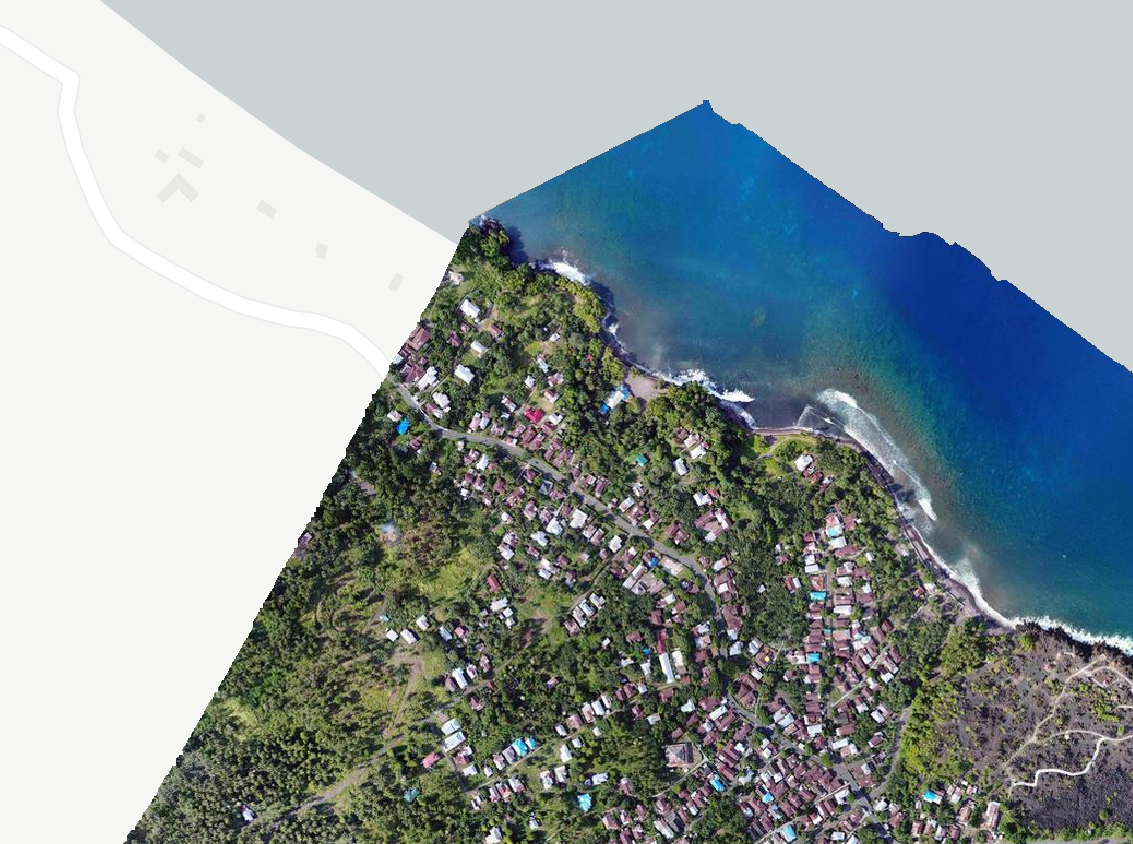
\includegraphics[width=\linewidth]{figs/orthomosaic.png}
  \caption{Orthomosaic. source: Indonesian Redcross/OpenAerialMap}
  \label{fig:orthomosaic}
\end{figure}


\section{Aerophotogrammetry}

Aerophotogrammetry takes the job on step further. 
%
By knowing the camera's intrinsic parameters, software are capable of matching a number of pictures, detecting features on the environment, and locating the point used to take each of the pictures, this process is called multi-view stereo. 
%
With this information, it is possible to rebuild in 3D most of the environments, enabling the operator to interact with the area as a 3D mesh.
%
By using precise GPS information(such as RTK/PPK\footnote{Real-Time Kinematics and Post-Processing Kinematics, two techniques fot increasing GPS accuracy.} data, or total stations) or known landmarks, it is possible to accurately measure distances, areas, volumes, angles and elevations, simplifying the surveyors' job.
%
Aerophotogrametry can also be used to rebuild in 3D buildings and other structures, enabling precise calculations of volume and distances, allowing the use of 3D models on CAD software for faster and easier construction and planning.
%
It allows, for example, the calculation of displaced volume on a quarry, or how much landfill is required to level some terrain.
%

The results of an open-source multi-view stereo pipeline implementation using openMVS\cite{openmvs} and openMVG\cite{openmvg} can be seen on figures \ref{fig:cameras} and \ref{fig:church}. 
%
On figure \ref{fig:cameras} the software shows the cameras found, and their relative positions on the map. 
%
The orange areas are locations not covered by the cameras. 
%
It is important to notice that, as the coverage does not catch every angle of the structures, some deformations are expected, especially on hidden areas. 
%
Figure \ref{fig:church} shows the rebuilt and textured 3D model.
 
 \begin{figure}
\centering
  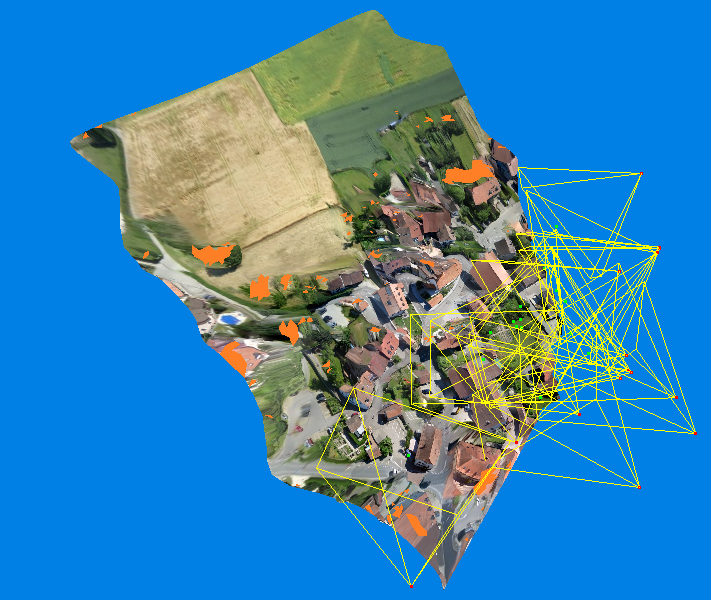
\includegraphics[width=\linewidth]{figs/cameras.png}
  \caption{Identified camera positions on "Oblique mapping of a village" dataset\cite{datasets}. }
  \label{fig:cameras}
\end{figure}


 \begin{figure}
\centering
\begin{subfigure}{.5\textwidth}
  \centering
  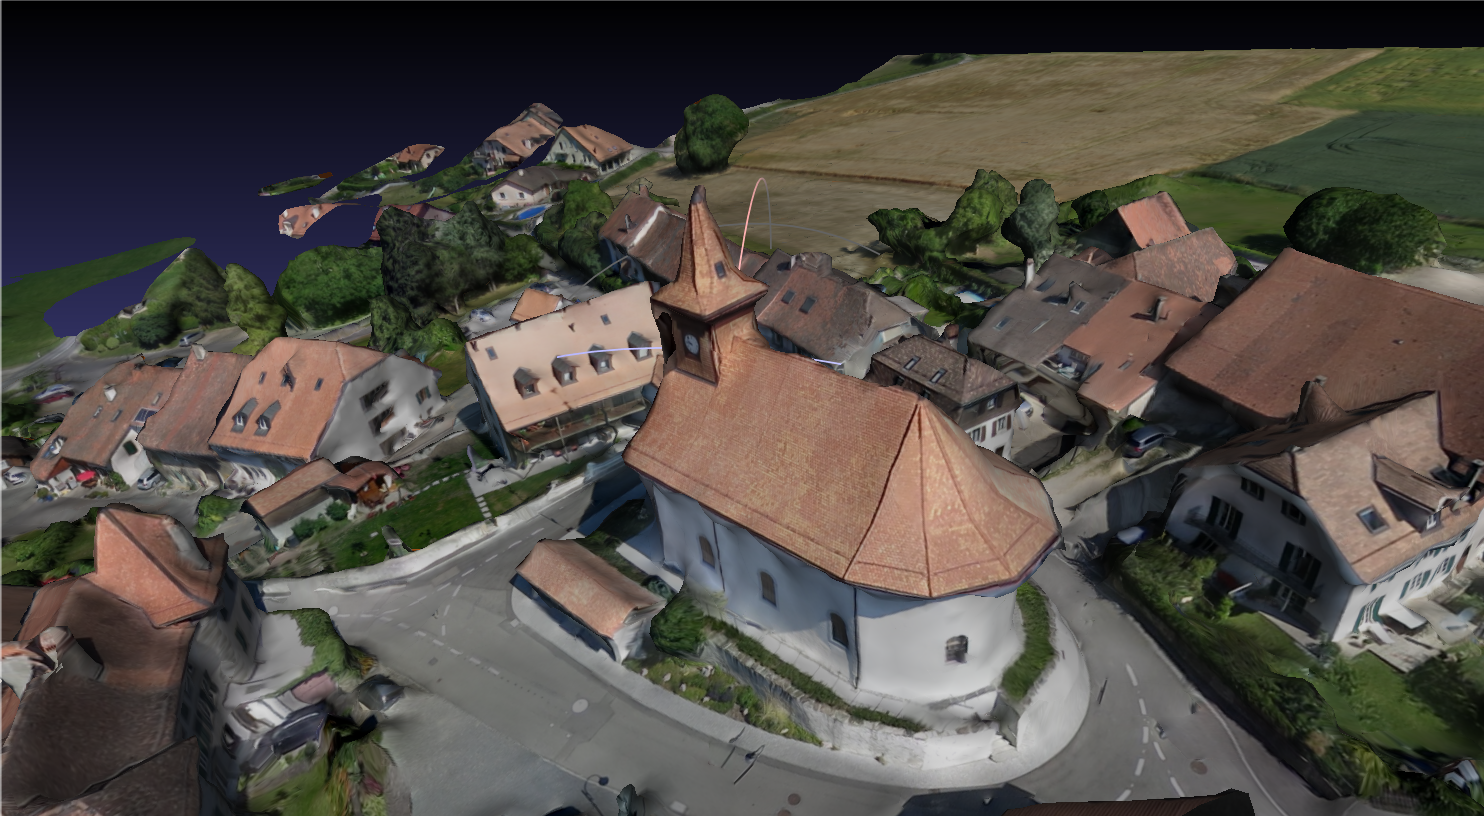
\includegraphics[width=\linewidth]{figs/church1.png}
  %\caption{Todos os passos do Nelder-Mead}
  
\end{subfigure}%
\begin{subfigure}{.5\textwidth}
  \centering
  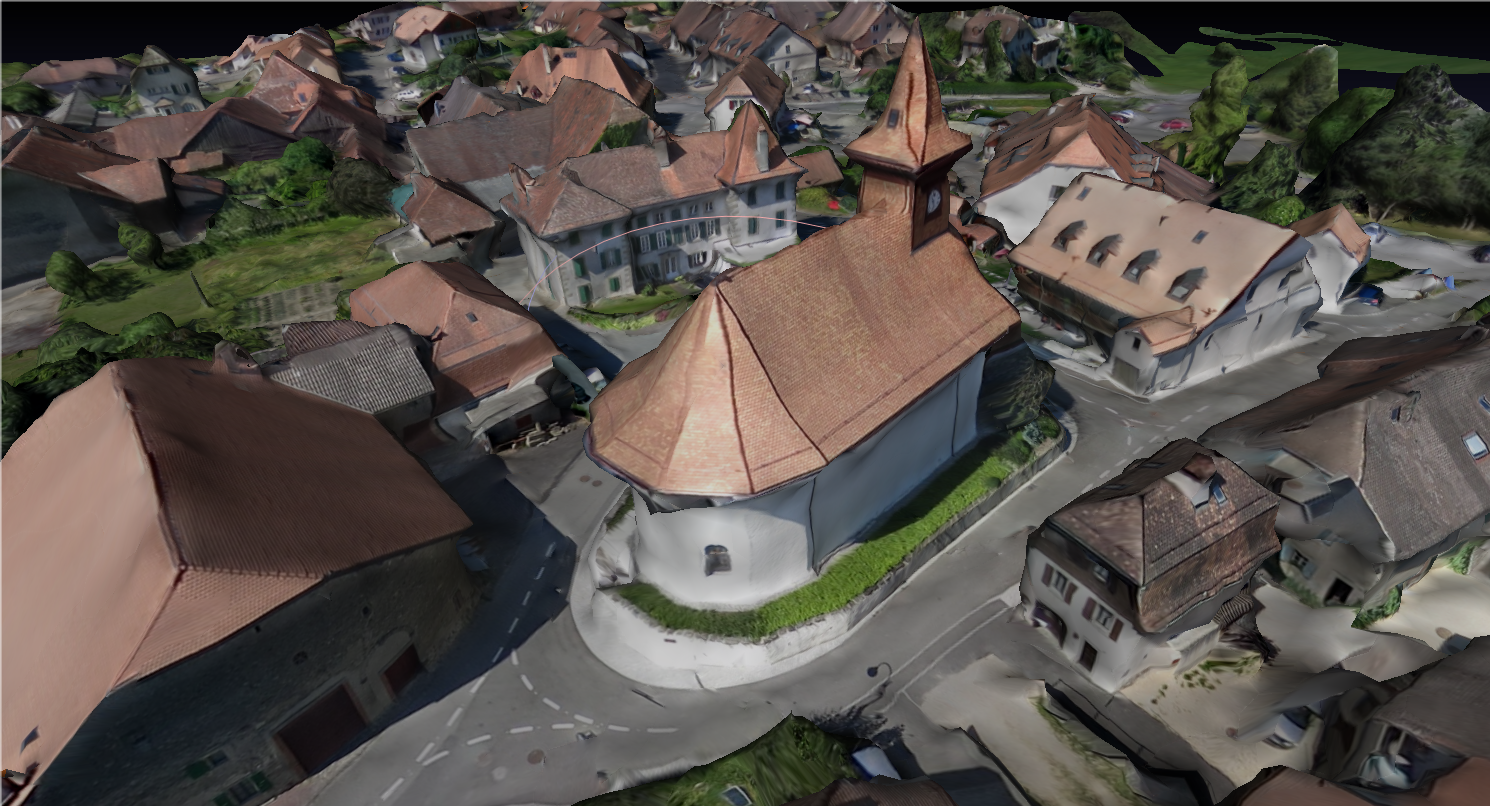
\includegraphics[width=\linewidth]{figs/church2.png}
  %\caption{Pontos avaliados pelo Nelder-Mead aplicado em um parabolóide.}

\end{subfigure}
\caption{3D reconstruction of the "Oblique mapping of a village" dataset\cite{datasets}.}
\label{fig:church}
\end{figure}



\chapter{Flight Mechanics and Design} \label{chap:FlightMechanics}

\section{Brief Introduction to Flight Mechanics}

Flight mechanics deal with a vehicles interaction with propulsional, aerodynamic, and gravitational forces.

In order to achieve proper flight, a vehicle needs an upwards force and means of maneuverability. the former is usually generated by the means of a propeller, while the latter can be either the result of spinning propellers or using control surfaces to deflect the passing air movement, causing a force to the opposite direction. 
%
Flight Mechanics is a field of mechanics which deals with the study of vehicle trajectories, performance, stability, and aerodynamic
control.


\section{Fixed-Wing Mechanics}

In fixed-wing aircraft, air flowing through the wings generates a pressure differential, usually lowering the pressure on top of the wing, generating a force usually called "lift", the force responsible for canceling the gravitational pull and keeping the vehicle aloft in the air.

In a simplified explanation, two main principles are responsible for generating lift:

\subsection{Flow deflection and Newton's laws}

Most wings have an angle of attack (to be hereafter called $\alpha$ ) such that $\alpha > 0$, which means the air passing through it gets deflected down. According to Newton's second law, an opposite force is necessary on the wing. This force is the generated lift.

\subsection{Increased flow speed and Bernoulli's principle}

Bernoulli's principle states that within a steady airflow of constant energy, when the air flows through a region of lower pressure it speeds up and vice versa. Implying there is a direct mathematical relationship between the pressure and the speed, meaning if one knows the speed at all points within the airflow, on can calculate the pressure and vice versa. For a cambered airfoil (where the chord at the top is longer that the chord at the bottom) the air needs to take a longer path, moving faster, thus lowering the pressure on the top, and generating lift.


\subsection{Airfoil Shape}
How much lift is generated depends on the chosen airfoil.
%
An cambered airfoil (longer chord on the upper surface than in the lower one) generated lift even when the angle of attack $\alpha$ is zero.
Symmetric airfoils need a positive angle, and the lift is generated by deflecting the air downwards.
Other properties that depend on the airfoil shape are the drag (air force pushing against the direction of movement) and angular moment it generates on the aircraft. 

\subsection{The Coordinate System and Nomenclature}

The coordinate system, when dealing with the fixed-wing and VTOL modes, is as shown in figures \ref{fig:coords1} and \ref{fig:coords2}.

\begin{figure}[h]
\centering
  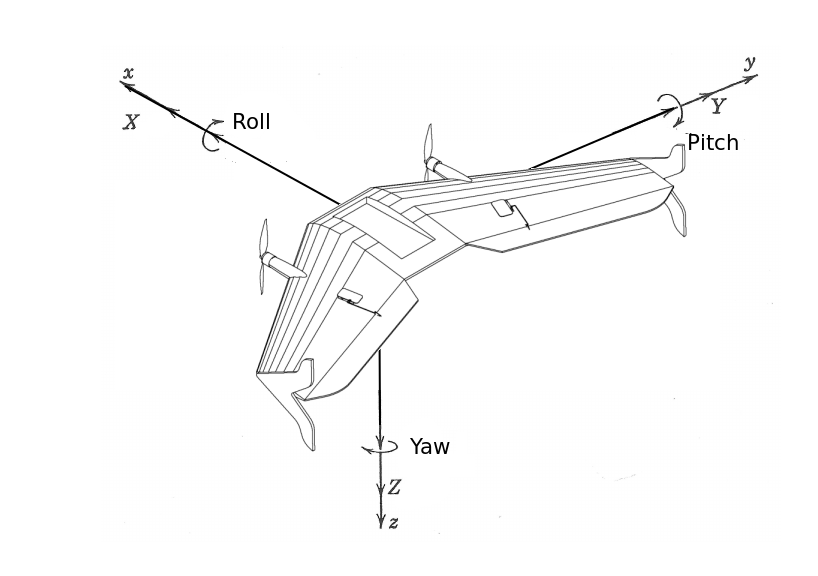
\includegraphics[width=0.8\linewidth]{figs/axisfixedwing.png}
  \caption{Coordinates system and relevant variables in fixed wing mode.}
  \label{fig:coords1}
\end{figure}


\begin{figure}[h]
\centering
  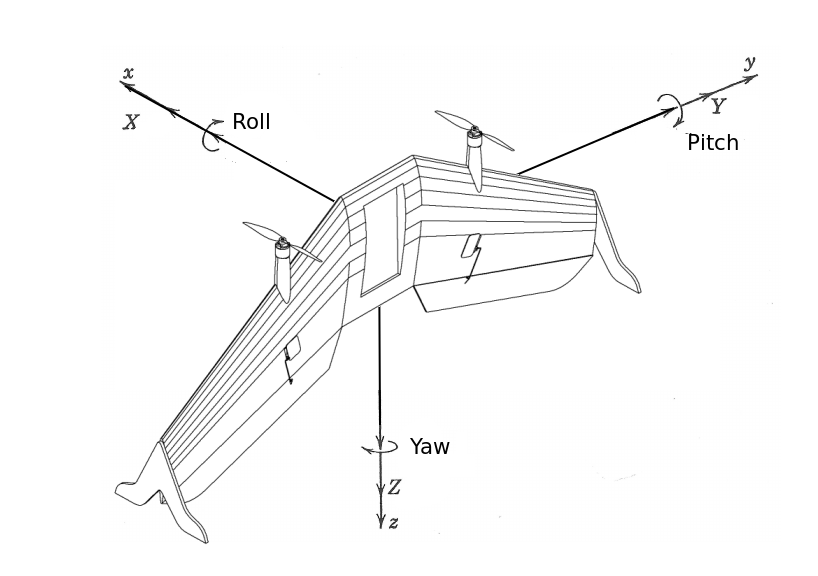
\includegraphics[width=0.8\linewidth]{figs/axisvtol.png}
  \caption{Coordinates system and relevant variables in VTOL mode.}
  \label{fig:coords2}
\end{figure}

Where:


\begin{itemize}

\item $x$, $y$, and $z$ are the coordinates, with the origin in the vehicle's center of mass.
%\item $u$, $v$, and $w$ are the linear velocities in each of the $x$, $y$, and $z$ coordinates, respectively.
\item $X$, $Y$, and $Z$ are the components of the aerodynamic force in each of the $x$, $y$, and $z$ coordinates, respectively.
\item Roll, Pitch and Yaw respectively represent the rotations around the X, Y, and Z axis.
\item Between VTOL and Fixed Wing mode, Yaw is Switched with Roll, as the controls switch to Multicopter mode, which usually have the rotors parallel to the ground.
%\item $p$, $q$, and $r$ are the linear velocities in each of the $x$, $y$, and $z$ coordinates, respectively.
%\item $u$, $v$, and $w$ are the linear velocities in each of the $x$, $y$, and $z$ coordinates, respectively.
%\item  Although not indicated in the figure, the variables $\phi$, $\theta$, $\psi$ represent the angular rotations,
%relative to the equilibrium state, about the x, y, and z axes, respectively. Thus, $p=\dot{\phi}$, $q = \dot{theta}$
%and $r = \dot{\psi}$ where the dots represent time derivatives.

%$\phi$, $\theta$, and $\psi$ can also be referred, respectively, as \textit{roll}, \textit{pitch}, and \textit{yaw}.

\end{itemize}

\section{VTOL Mechanics}

When in VTOL mode, the coordinate system used is similar to that in a conventional multirotor, with $Z$ pointing up parallel the motors axis, and $X$ going throughb the fuselage, pointing away from the belly of the aircraft.

The mechanics involved in vertical take-offs and landings is slightly different. The lift generated becomes meaningless, no more than a slight perturbation to the system. The generated thrust becomes directly responsible for vertical motion and roll control, while the control surfaces can redirect the airflow allowing control of yaw and pitch.

An approximate model can be seen on \cite{7487466}, where a wind-tunnel was used to find the parameters. As this work does not focus on the dynamics or control itself, it is not detailed here.


\section{XFLR5}

XFLR5 is an analysis tool for airfoils, wings and planes operating at low Reynolds Numbers. It includes:
\begin{itemize}

\item XFoil's Direct and Inverse analysis capabilities;
\item Wing design and analysis capabilities based on the Lifting Line Theory, on the Vortex Lattice Method, and on a 3D Panel Method.

This tools enables the iterative design and analysis of multiple aircraft configurations.

%\todo{elaborar aqui}

\end{itemize}


\section{Design}

The chosen design is the one of a flying wing, a fuselage-less aircraft made of a wing, propulsion system, and control surfaces. The reasons are because of a simpler and sturdier mechanical structure, besides the possibility of the VTOL configuration.

\subsection{Preliminar Design}

As a starting point, a wing with a central hub and 2 semi-wings ending in symmetrical winglets was designed. The ZAGI12 airfoil was chosen due to it's good soaring capabilities and low stall speed.
%\todo{citation needed}.

With the airfoil chosen, It's characteristics were calculated with the aid of XFOIL, an airfoil analysis tool built into XFLR5.

\begin{figure}[h]
\centering
  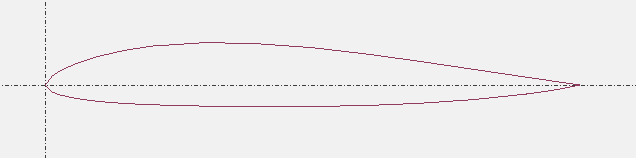
\includegraphics[width=\linewidth]{figs/zagi12.png}
  \caption{Zagi 12 airfoil.}
  \label{fig:zagi12}
\end{figure}


These characteristics plots can be seen on figure \ref{fig:zagi12polares}.
%

From this figure, the point with the highest Cl/Cd ratio, the theoretical point with better lift to drag ratio, and therefore best gliding performance can be found. It's also notable that the airfoils moment "pulls" it into this better Cl/Cd ratio, allowing the aircraft to fly into this ideal condition without deflection of the control surfaces, which would cause aerodynamical losses.


\begin{figure}
\centering
  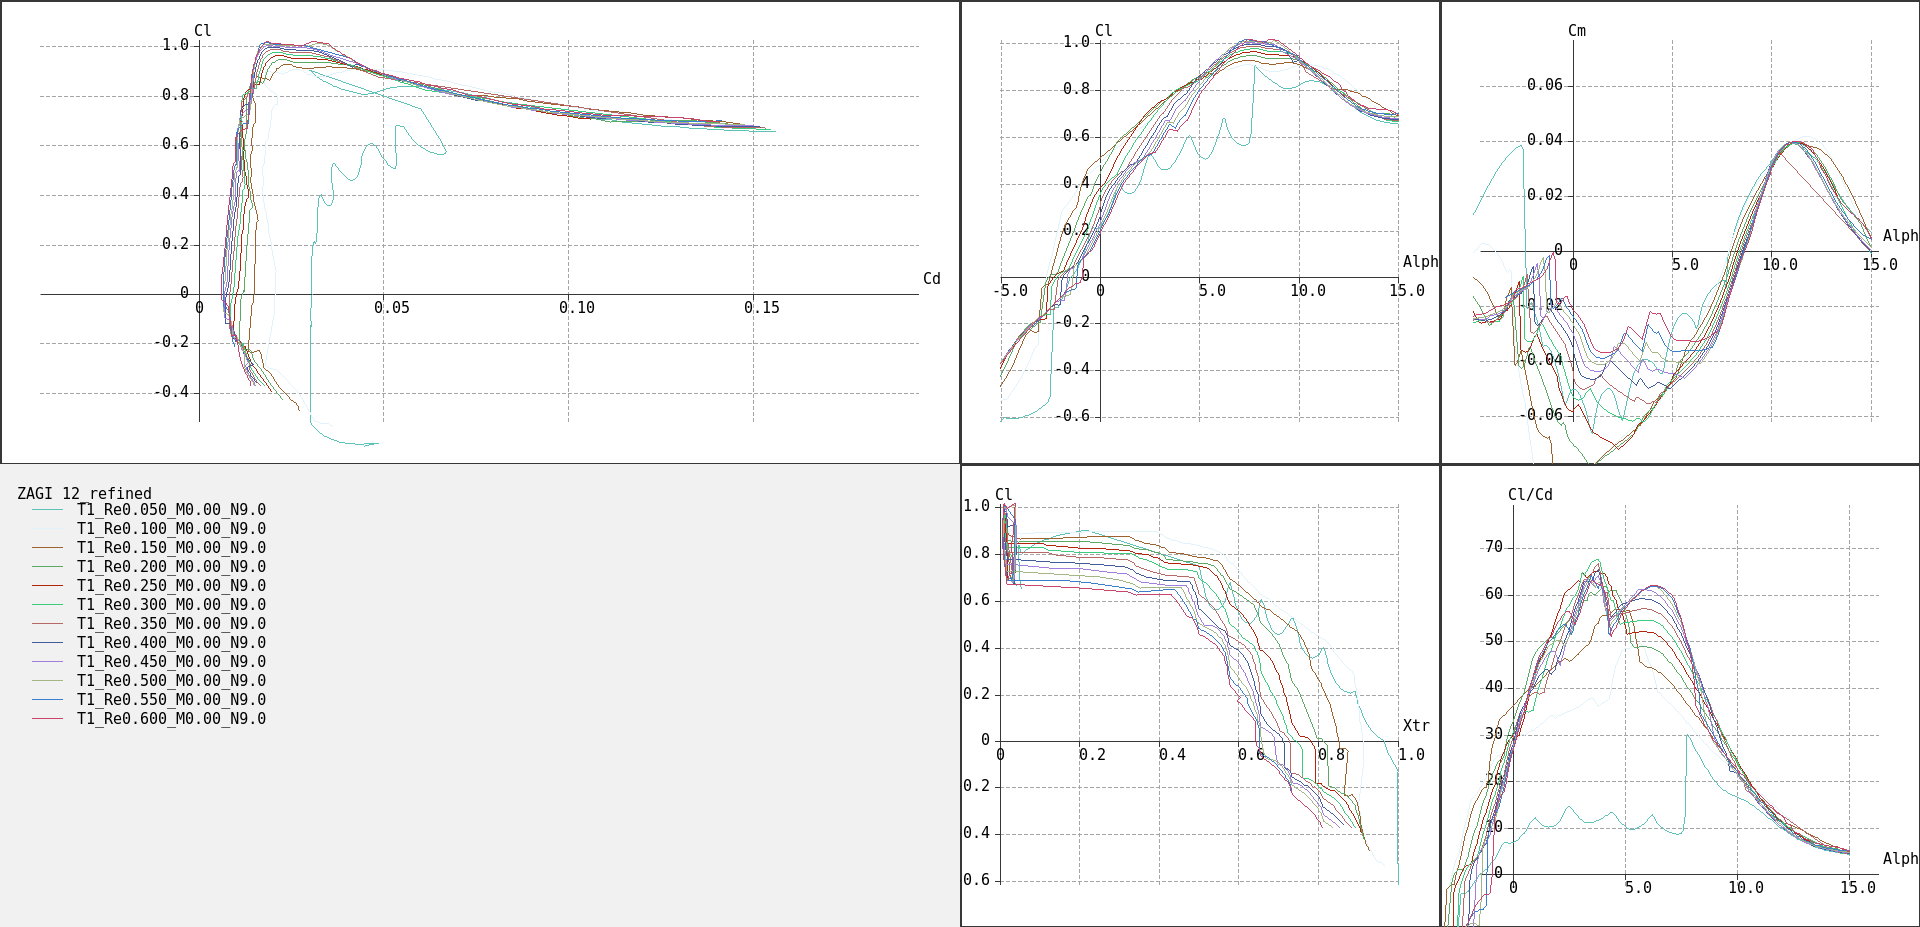
\includegraphics[width=\linewidth]{figs/polares.png}
  \caption{Zagi 12 characteristics}
  \label{fig:zagi12polares}
\end{figure}

With that data, the main body was conceived, as seen in the figure \ref{fig:preliminar}. With this CAD tool we can then analyze the performance of the aircraft as a whole. This gives us the same data as the airfoils', but for the whole craft, as seen in figure \ref{fig:craftpolar}.

More data can be inferred from these graphs. From \ref{fig:zagi12polares} it can be seen that the highest $C_l$, or Lift Coefficient, is obtained around $\alpha = 8\deg$, which, possibly by design of the airfoil, is also the zone with a higher $C_l/C_d$, or \textit{lift-to-drag ratio} maximizing the gliding distance. It's also notable tat the $C_m  \times \alpha$ plot crosses 0 around the the same $8\deg$, meaning the profile is generally trying to point at that angle.

\begin{figure}
\centering
  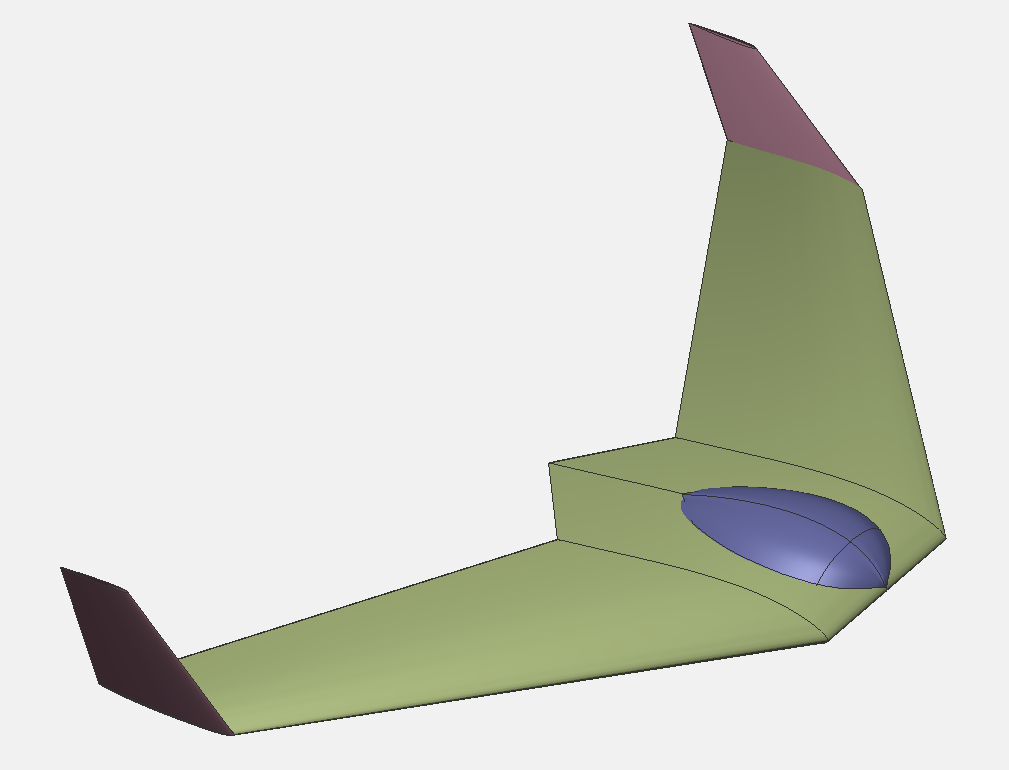
\includegraphics[width=\linewidth]{figs/preliminar.png}
  \caption{First concept of the aircraft.}
  \label{fig:preliminar}
\end{figure}


From \ref{fig:craftpolar}, it is noticeable that without command inputs, the aircraft tends to point the nose down $ 2 \degree $ , reaching it's maximum lift-to-drag ratio and slowly coming back to the ground. It is good to notice that the comprehensive simulation of the aircraft takes into account the center of mass, making it possible to make the aircraft to fly straight with no input, instead of pointing slightly downwards, by changing the center of gravity slightly to the trailing edge. This change would, however, decrease the stability of the aircraft and increase the chances of a stall.

\begin{figure}
\centering
  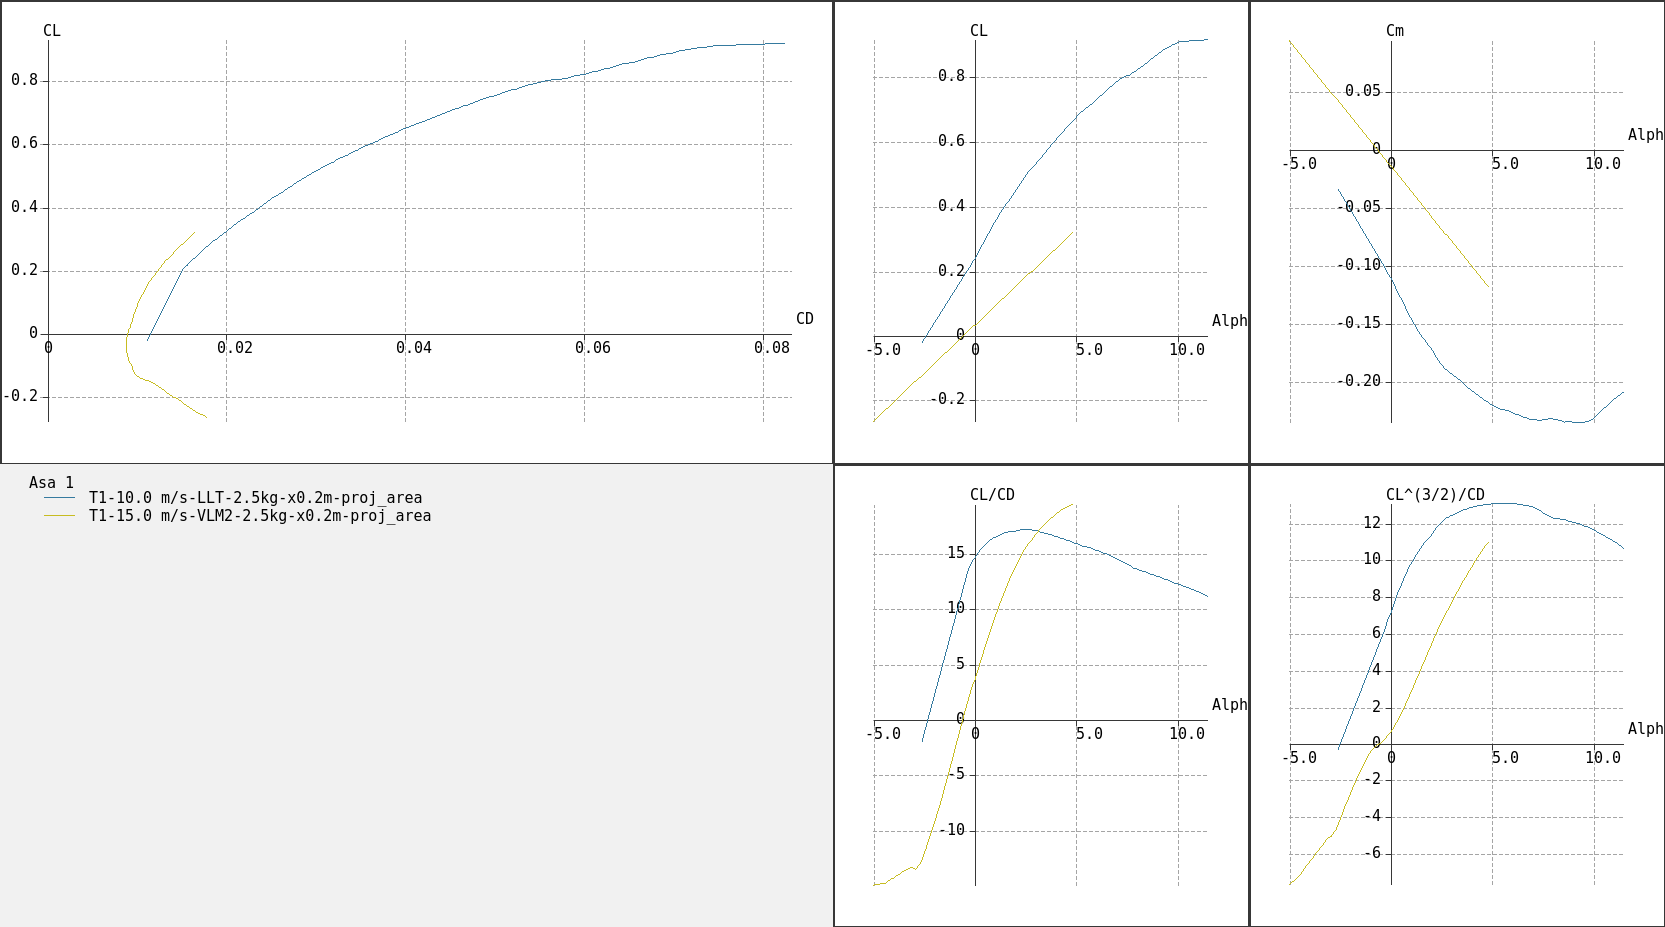
\includegraphics[width=\linewidth]{figs/craftpolar.png}
  \caption{Flight characteristics of the preliminary aircraft design.}
  \label{fig:craftpolar}
\end{figure}


\subsection{Final Design}

Due to building issues and the desire to maximize both effective payload and flight autonomy, the design was simplified, extending the chord back on the beginning of the wings, as seem on figures \ref{fig:final} - \ref{fig:finalrendertop}.
The electronics bay was embedded into the main section, reducing the aerodynamical cross-section, thus reducing drag. The whole design was then assembled on Autodesk Inventor Professional prior the manufacturing of the prototype.
	

\begin{figure}
\centering
  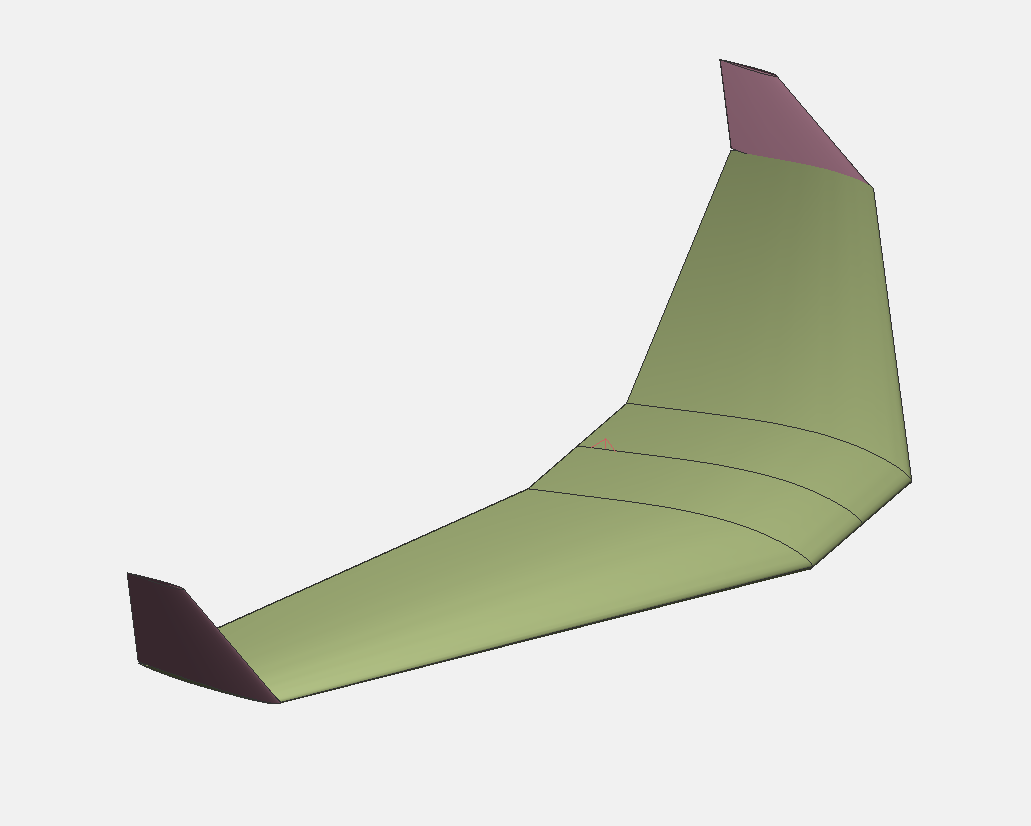
\includegraphics[width=\linewidth]{figs/final.png}
  \caption{Final design of the aircraft, on XFLR5.}
  \label{fig:final}
\end{figure}
	
\begin{figure}
\centering
  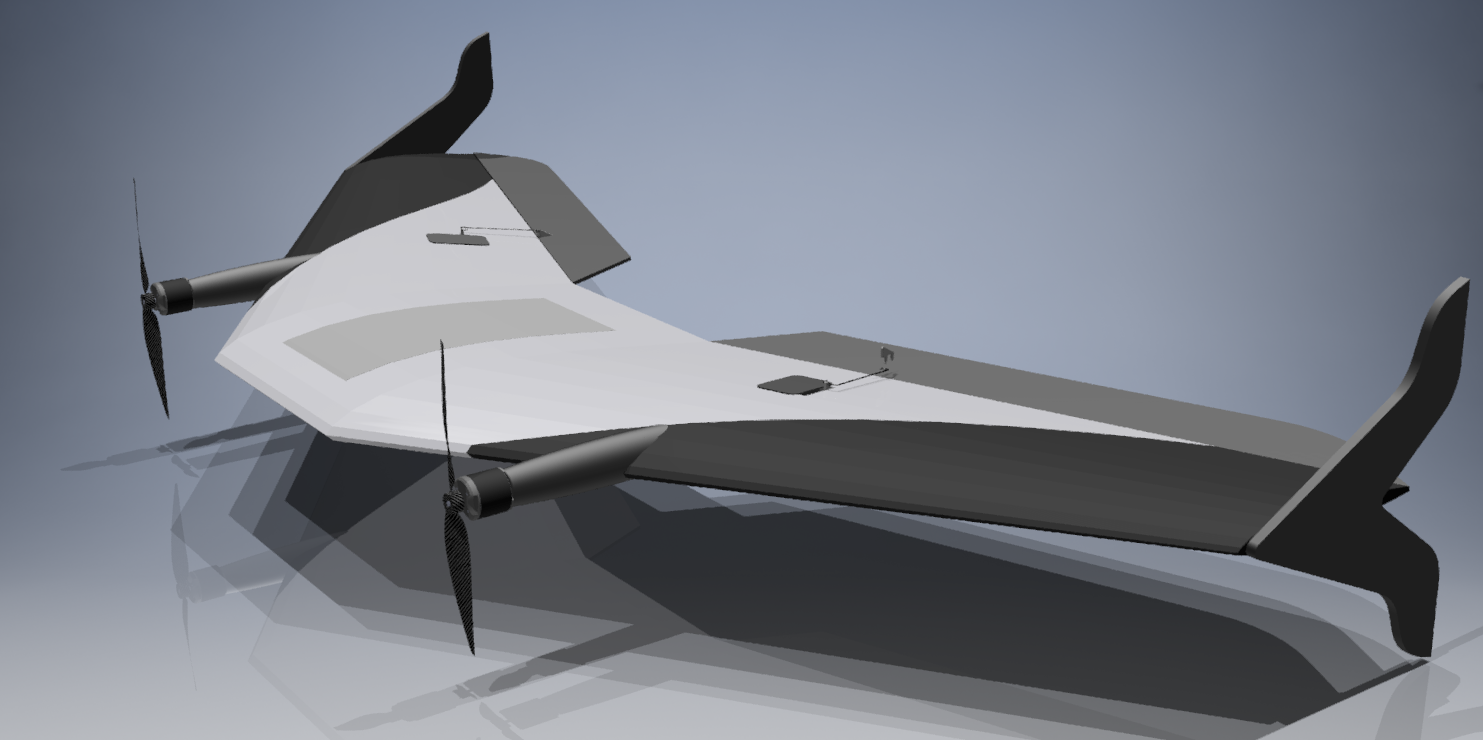
\includegraphics[width=\linewidth]{figs/finalrender.png}
  \caption{Final design of the aircraft.}
  \label{fig:finalrender}
\end{figure}

\begin{figure}
\centering
  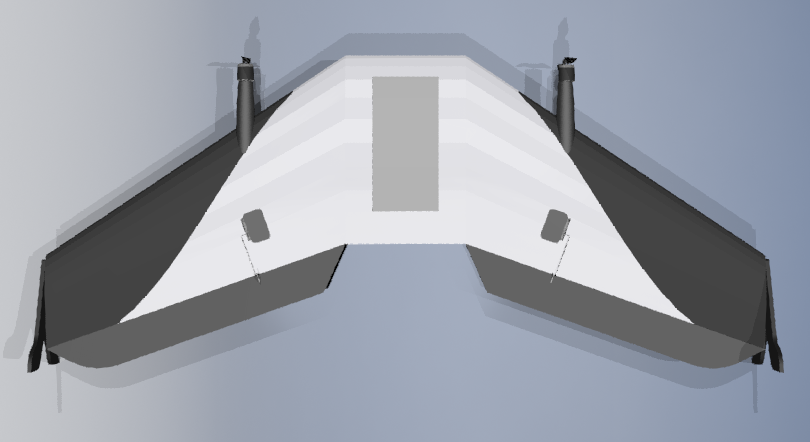
\includegraphics[width=\linewidth]{figs/finalrendertop.png}
  \caption{Final design of the aircraft, top view.}
  \label{fig:finalrendertop}
\end{figure}


%%%%%%%%%%%%%%%

\chapter{The Eletronics} \label{chap:electronics}

In order for the aircraft to fly and navigate autonomously, onboard electronics are required, for both actuation, power source, and navigation. Some of the used electronics were already available, and were chosen for this reason.
	
\section{Propulsion}

Due to the familiarity and availability, the Mikrokopter Mk3538 Motor was chosen, paired with E-Max Simon 60A escs.

Experimental curves for the motor are available at Mikrokopter's website, and the relevant ones are reproduced on Figure \ref{fig:motorcurves}. Each motor should give, on 16 V, around 1.9 kg of static thrust when paired to 12 inches propellers, up to 2.5 kg on 15 inches, while drawing 35 A, or about 560 W.

\begin{figure}[H]
\centering
  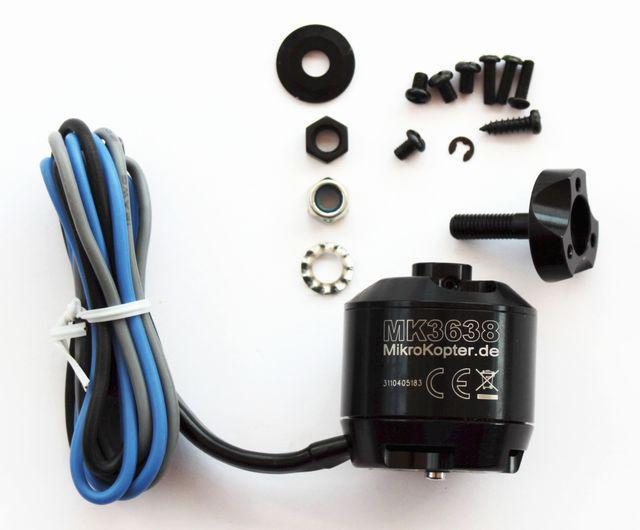
\includegraphics[width=0.8\linewidth]{figs/mk3638.jpg}
  \caption{Mikrokopter MK3638 Brushless Motor.}
  \label{fig:yaw_loop}
\end{figure}

\begin{figure}[h]
  \centering
  \begin{subfigure}{.8\textwidth}
    \centering
    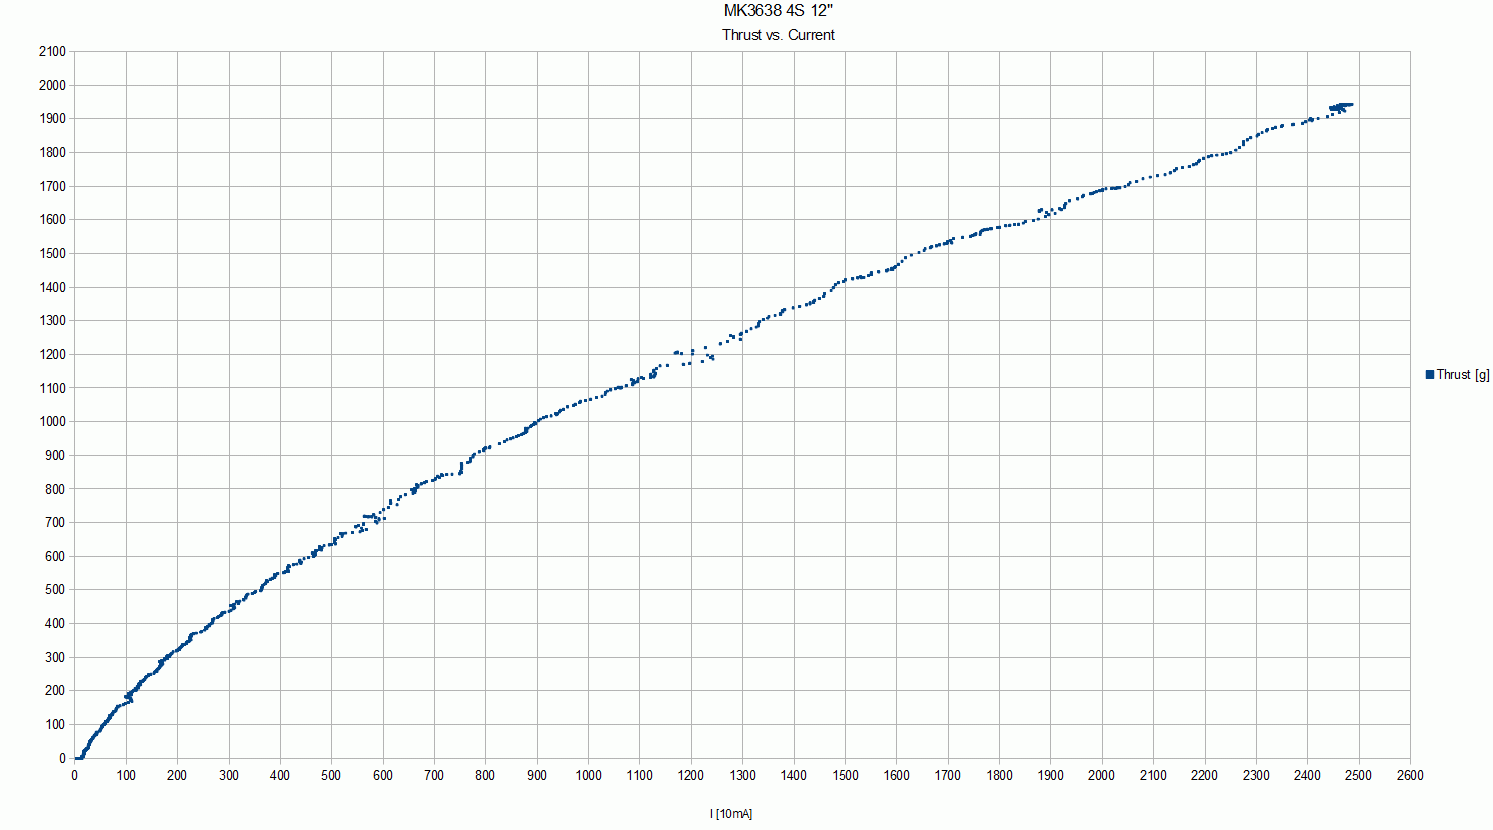
\includegraphics[width=\linewidth]{figs/curve12.png}
  
  \end{subfigure}%
  
  \begin{subfigure}{.8\textwidth}
    \centering
    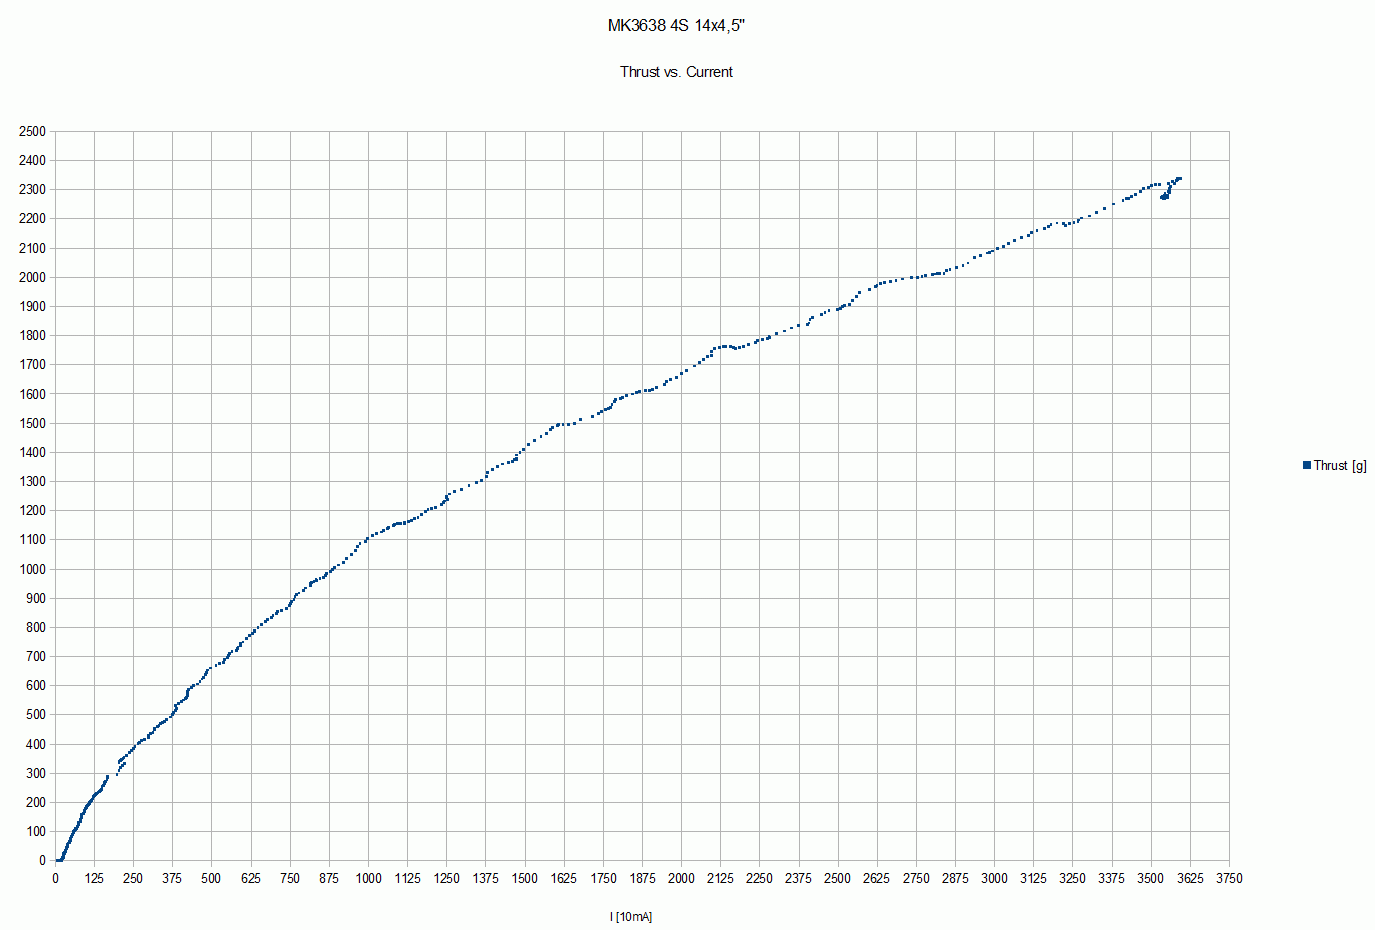
\includegraphics[width=\linewidth]{figs/curve15.png}

  \end{subfigure}
  \caption{Motor curves with 12 and 15 inches propellers.}
  \label{fig:motorcurves}
\end{figure}


As the airplane is aimed to weigh around 3 kg, each motor needs to pull at least 1500g for hovering, leaving a maneuvering margin of around 1 kg for each motor.

\section{Batteries}

As each motor can draw up to 35 A, the battery should be able to provide up to 70 A without issues.
The Batteries chosen are also the ones already in use by the company, Multistars 10000 mAh 10C, which, at 10 C rating, are able to sustain a constant draw of up to 100 A. 

Each weigh approximately 750 g and measures XXxYYxZZ mm.
\todo{medir}

\begin{figure}[H]
\centering
  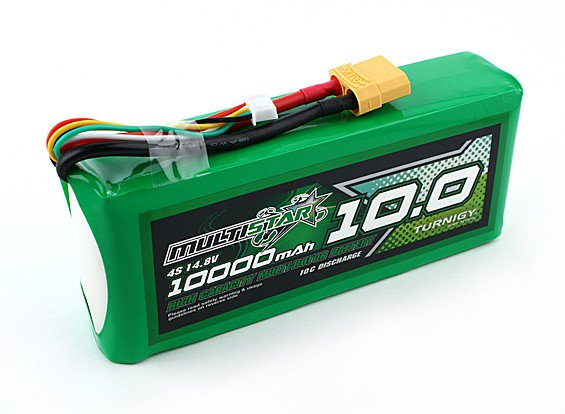
\includegraphics[width=0.8\linewidth]{figs/battery.jpg}
  \caption{Multistar 4s 10000 mAh Lithium Polymer battery.}
  \label{fig:yaw_loop}
\end{figure}


\section{The Servos and Control Surfaces}

The control surfaces must be slightly larger than usual for a flying wing, as on a tail-sitter a reasonable amount of air must be deflected on hover situation, while on most wings a steady airflow is assumed. It's suggested to have control surfaces taking up to 30\% of the chord of the wings. Since they are easily swappable, it was decided to start with smaller ones, with a 10 cm chord, and replace them if necessary.


The servos chosen were standard servos Savox SV-0220, linked to the elevon horns with a stiff wire.

\begin{figure}[H]
\centering
  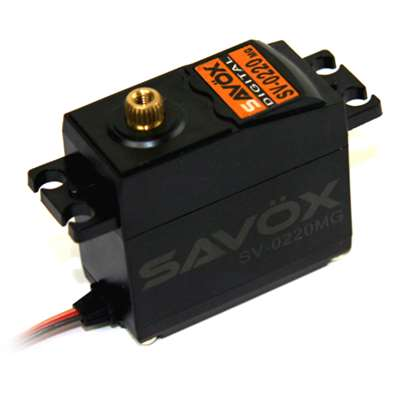
\includegraphics[width=0.8\linewidth]{figs/servo.jpg}
  \caption{Savox SV-0220 servo.}
  \label{fig:yaw_loop}
\end{figure}


\begin{table}[]
\centering
\caption{SV-0220 Technical Specifications}
\label{my-label}
\begin{tabular}{lll}
 Torque @ 6v &   6.5kg & \\
 Torque @ 7.4v & 8.0kg & \\
 Speed @ 6v    &  0.16 sec/60 deg & \\
 Speed @ 7.4v  &  0.13 sec/60 deg & \\
 Dimensions L x W x H (mm) &  40.7 x 20.0 x 37.0 & \\
 Weight & 59.0g &
\end{tabular}
\end{table}

\section{The Flight Controller}

The multirotor had a huge boom last 10 years. In 2009 the first hobby-grade flight controller for multicopters was born, Rolf "KaptainKuk" Bakke's "KK board". Using a simple AVR controller and three gyroscopes, the board could control angular speed on three axis, enabling pilots to control the multirotors. It was programmed in AVR assembly and had individual PID controllers for each axis.
%
Shortly after, Alexinparis noticed the gyros on the Wii Motion + controller, and MultiWii was born. This project grew to support a variety of sensors and boards, and had an active development community, but has now saturated the AVR controller's capability.
%
Shortly after, still in 2010, DIY Drones released the open-source Arducopter, featuring more advanced flight modes, and even autonomous flight.  It did still involve compiling code and flashing it to the controller though.
%
In 2011, DJI started to get visibility with the NAZA controller, which showed remarkable stability, and later got upgraded with a GPS allowing the drone to return to home and hold position in the air. The controller was often sold with a standard frame and motors, which improved stability as the board was pre-tuned to the sold equipment.

Shortly after DJI began to manufacture the DJI Phantom drones, which is now the main player in the market.
%
Nowadays, three major controllers coexist: MultiWii was ported to 32bits architecture processors and lives on as Baseflight and Cleanflight, mostly on quadcopter racing boards; DJI leads the aerial photography market with their phantom quadcopters; And on the autonomous fields, Ardupilot, PX4, Mikrokopter, and DJI are still competing for the better solutions.


The Flight Controller board chosen is a PixHawk. Both PX4 and ArduPilot stacks support this board. But Ardupilot is a more mature, tested, open, and community-based platform, and thus it was chosen here, running latest release of ArduPlane, where there's experimental support for tail-sitters.

\begin{figure}[H]
\centering
  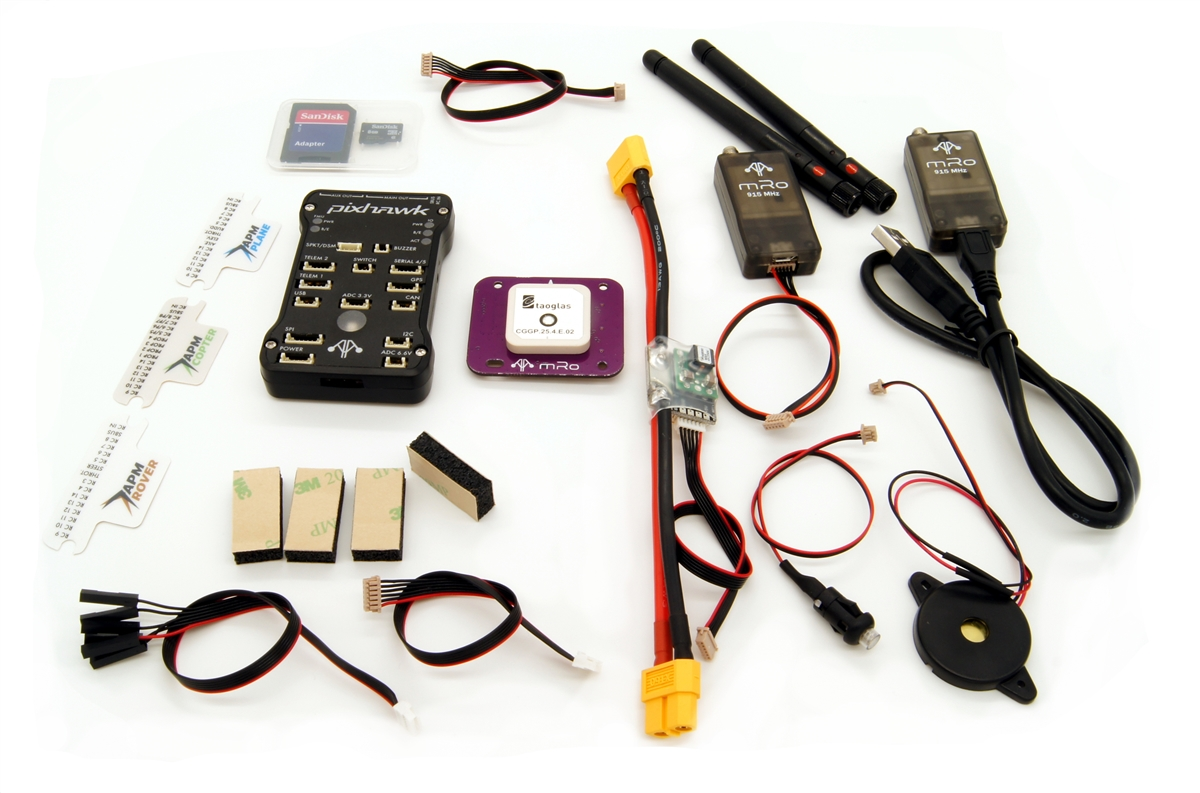
\includegraphics[width=0.8\linewidth]{figs/pixhawk.jpg}
  \caption{Pixhawk flight controller and most peripherals. Source: Mrobotics}
  \label{fig:pixhawk}
\end{figure}

\section{The GPS}
The used GPS is a U-Blox M8N GPS receiver, coupled with an external compass sensor. The external compass is important because the high currents flowing close the Pixhawk affect the readings of the internal compasses.
%
It supports concurrent reception of up to 3 GNSS (Global Navigation Satellite Systems), GPS, Galileo, GLONASS and BeiDou.

It's precision is around 3 m, occasionally getting lower than 1 m\cite{m8ntest}.

\begin{figure}[H]
\centering
  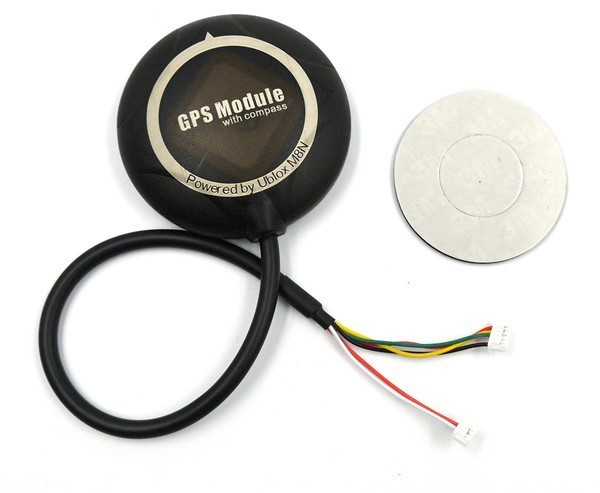
\includegraphics[width=0.8\linewidth]{figs/m8n.jpg}
  \caption{M8N GPS receiver and external compass. Source: cooltoyz.co.uk}
  \label{fig:m8n}
\end{figure}


\section{The Telemetry}

The telemetry system provides a serial (UART) connection to the aircraft, via a radio system.
%
The one used can be seen on the top right corner of Figure \ref{fig:pixhawk} and is a 900Mhz radio modem.
%
The telemetry allows real-time reading of parameters and attitude, as well as writing them for setup and tuning.

\section{The Radio Control System}

The used Radio System is a 2.4Ghz radio by Turnigy, the Turnigy 9x.
%
This radio uses fast frequency hopping to avoid interference, and has a reported range of up to 3 km \cite{range9x}.
%
The radio was modded\cite{t9xmod} and the firmware was replaced by the open-source OpenTX \cite{opentx}, which provides much more flexibility to the system, as custom mixes, switches, automatic functions, periodic functions, and telemetry capabilities.

\begin{figure}[H]
\centering
  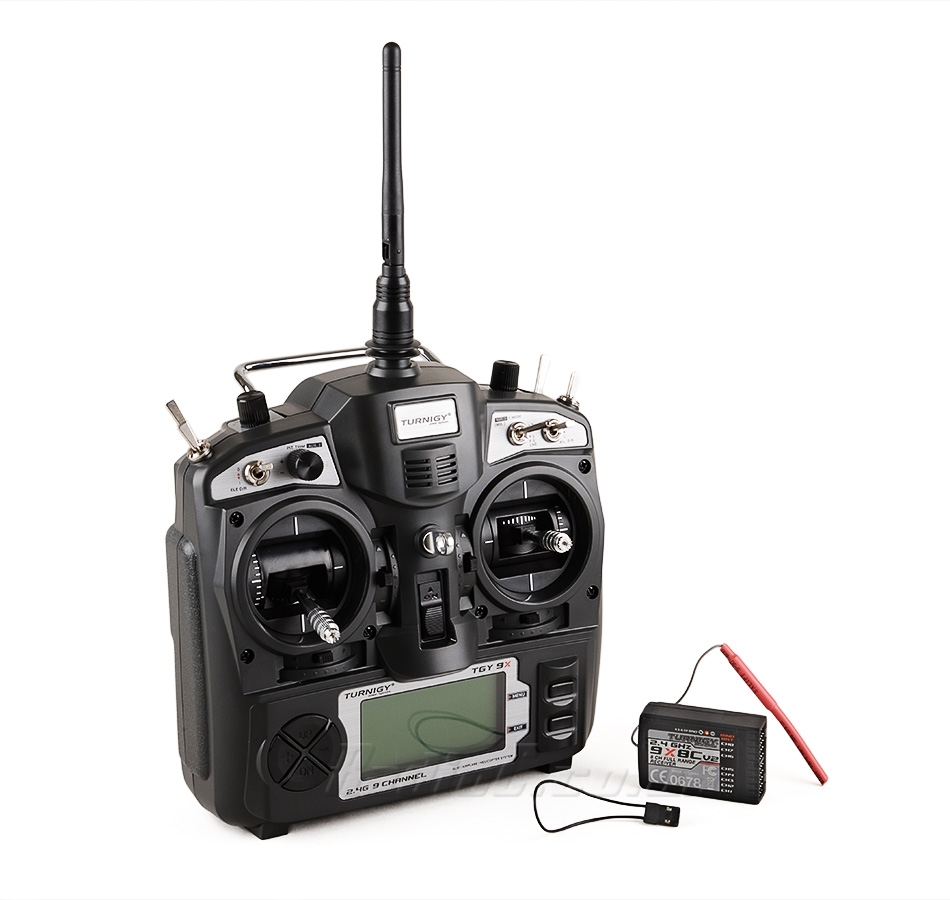
\includegraphics[width=0.8\linewidth]{figs/t9x.jpg}
  \caption{The Turnigy 9X Radio System. Source: radioc.co.uk}
  \label{fig:t9x}
\end{figure}


%%%%%%%%%%%%%%%%%%%
\chapter{The Software}

Two main types of software are required for the operation of this kind of aircraft. The flight controller runs on the on-board computer and is responsible for controlling the flight itself, and a ground station software, responsible for higher level commands and telemetry.
This chapters details these software used in the project.

\begin{figure}[h]
  \centering
  \begin{subfigure}{.5\textwidth}
    \centering
    
\includegraphics[width=\linewidth]{figs/px4.png}
  \end{subfigure}%
  \begin{subfigure}{.5\textwidth}
    \centering
    
\includegraphics[width=\linewidth]{figs/ardupilot.png}

  \end{subfigure}
  \caption{PX4 and Ardupilot.}
  \label{fig:motorcurves}
\end{figure}


\section{Flight Controller}
The flight controller software runs on the on-board computer, and is responsible for controlling the attitude, altitude, and position of the aircraft.
%
In order to achieve this, most flight controller boards come with internal sensors (accelerometer, gyroscope, magnetometer, barometer) and external ones (airspeed, magnetometer, GPS). 
%
The acquired data is used to estimate attitude and position, which is then corrected by the control loops.

The possible choices of flight controller software were ArduPilot and PX4.
%
Ardupilot is a community-drive software started by DYIDrones in 2009\cite{diydrones}.
%
It's GPL licensed, which means all changes made and commercialized must be open-sourced\cite{gplv3}.
%
ArduPilot is a mature software, with a large community of users and testers.
%
%https://github.com/PX4/Firmware/commits/master?after=3e0b8b7016556224aedb54f51d769d3288f0920e+24770

PX4 was also developed since 2008[\cite{waybackmachine}, mostly by the Computer Vision and Geometry Lab of ETH Zurich (Swiss Federal Institute of Technology)\cite{computervision} and the Autonomous Systems Lab\cite{autonomouslab} under a more permissive BSD 3-clause license\cite{bsd}.
%
For a while both projects worked closely, the Pixhawk Flight Controller board is a result of this interaction.
%
Both also joined Dronecode\cite{dronecode}, a Linux Foundation\cite{linuxfoundation} initiative started in 2004 as an attempt to grow the UAV ecosystem and reach larger companies.
%

Dronecode however, evolved into, according to the Ardupilot Dev Team, a flawed model.
%
It was required for all projects to hand over all domains, accounts, and trademarks to their control.
%
The project are also directed by the so-called "Platinum Members", which means the development would not be in control of the community anymore.
%
By September 9, 2016, a letter was released stating that Ardupilot was leaving Dronecode, and explaining why\cite{letter}.

The Ardupilot code was chosen for this project due to their larger openness and community.


\chapter{The Control Structure} \label{chap:control}

The control Structure used is the one of ArduPlane. In hover, or tail-sitter mode, the ArduCopter stabilization system is used, while in airplane/fixed-wing mode, Arduplane’s controllers are used. Both will be discussed and explained in the following sections.

\section{The Data Acquisition}

In order to control all the required variables, they must be available for the controller. The Pixhawk controller provides two redundant IMUs for this reason. Each of them runs an Extended Kalman Filter tracking 22 states\cite{kalman}\cite{kalmanArducopter}. Of the two running Kalman Filters, the one with smaller error estimation is used, and the estimated states are made available for the controllers.

\section{On Airplane Mode}

On Airplane mode, the aircraft is always moving forward, towards the $X$ axis, position control depends on defining a route and pointing the aircraft in order to remain on it.

\subsection{Roll and Pitch Control}

The roll and pitch control loops (seen in figures \ref{fig:roll_loop} and \ref{fig:pitch_loop}) are responsible for keeping the aircraft on the desired orientations on the $X$ and $Y$ axis. Usually, pitch is controlled by turning the elevator up and down, while roll is controlled by the deflecting the ailerons. On this aircraft, however, there are only two control surfaces, such that the output of both controllers are summed (\texit{mixed}, as is usually said in the RC world) in order to control both axis at the same time.
While at first they look like a classical P+I+D controller, there are some small changes:

\begin{itemize}
\item There's a feedforward controller trying to cancel the current angular rates.
\item The Derivative and Integral terms are scaled to the airspeed, and the controller's output as well. This is because  as the aircraft moves faster, less deflection is necessary to displace the same amount of air, resulting in the same movement of the body.
\end{itemize}


The controller outputs are called AileronDemand and ElevatorDemand, and are the theoretical required input on each axis. Ardupilot works like this in order to abstract the possible airframes. The next code stage mixes these needs to get the proper output for the current airframe.
On an airplane, the outputs are only limited to the maximum and minimum possible outputs, on an aircraft like the one in this project, the outputs are summed and subtracted to get the correct outputs on each elevon.


\begin{figure}[H]
\centering
  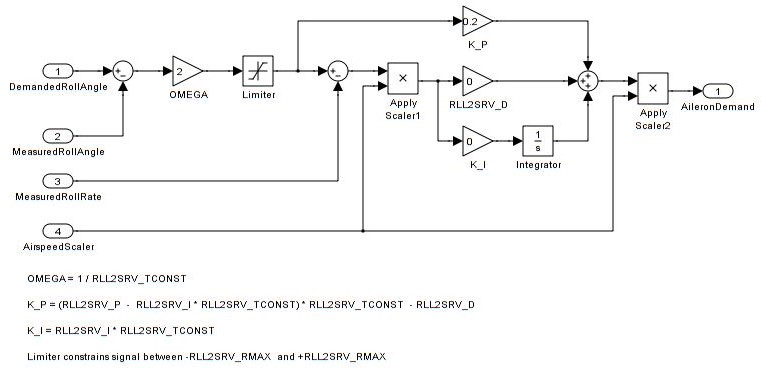
\includegraphics[width=\linewidth]{figs/roll_control_loop.jpg}
  \caption{Roll control loop. Source: ArduPilot}
  \label{fig:roll_loop}
\end{figure}

The transfer function for RollDemand is as follow:

\begin{equation}
D_{ail}(s) = \bigg(\frac{A_s(s) K_p s + A_s(s)^2(K_d s + K_i)}{s}\bigg)(\overline{R}(s) - R(s)) - A_s^2(K_D s + K_i)Rs
\end{equation}
\begin{equation}
R(s) = \Omega sat(R_{raw}(s))
\end{equation}

Where $R_{raw}(s)$ is the raw roll reading, $D_{ail}(s)$ is the aileron demand, $A_s(s)$ is an airspeed scaling value, $0 < A_s < 1$ (responsible for reducing the control outputs at higher speed, as most aerodynamical forces are proportional to the square of the airspeed), $K_d$ is a derivative term, $K_i$ is an integral term, $\overline{R}(s)$ is the Roll angle setpoint, and $R(s)$ is the current roll angle.


\begin{figure}[H]
\centering
  \includegraphics[width=\linewidth]{figs/PitchAP.jpg}
  \caption{Pitch control loop. Source: ArduPilot}
  \label{fig:pitch_loop}
\end{figure}

The transfer function for PitchDemand is similar:

\begin{equation}
D_{pit}(s) = \bigg(\frac{A_s(s) K_p s + A_s(s)^2(K_d s + K_i)}{s}\bigg)(\overline{P}(s) - P(s)) - A_s^2(K_D s + K_i)Ps
\end{equation}
\begin{equation}
P(s) = \Omega sat(P_{raw}(s)) + P_{2R}R(s)
\end{equation}

Where $P_{raw}(s)$ is the raw roll reading, $D_{pit}(s)$ is the aileron demand, $A_s(s)$ is the same airspeed scaling value, $K_d$ is the derivative term, $K_i$ is the integral term, $\overline{P}(s)$ is the Pitch angle setpoint, and $P(s)$ is the current pitch angle. Additionally, $P_{2R}R(s)$ is a term that attempts to cancel out the effect of banking the aircraft affecting the pitch.



\subsection{Yaw Control}
The Yaw Control loop controls the angle around the Z axis. This is usually used for landing only, and is not necessary on this aircraft on airplane mode. It can, however, be seen in figure \ref{fig:yaw_loop}.
Like the D and I terms on the roll axis, the controller's output is again scaled with the square of the \textit{AirspeedScaler} factor.
%\todo{dafuq?}

\begin{figure}[H]
\centering
  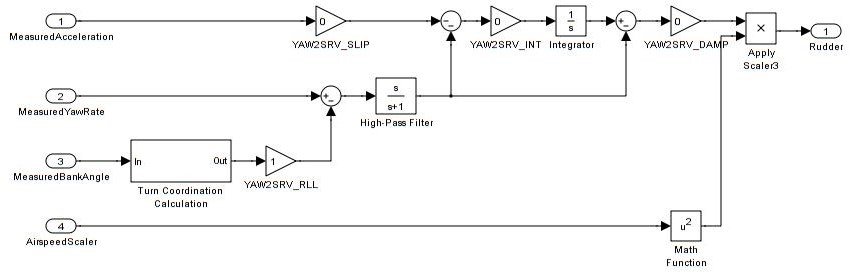
\includegraphics[width=\linewidth]{figs/yaw_control_loop.jpg}
  \caption{Yaw control loop. Source: ArduPilot}
  \label{fig:yaw_loop}
\end{figure}

The transfer function for RudderDemand is the following:

\begin{equation}
D_{rud}(s) = \underbrace{ - \frac{A_s^2 D_y K_i}{s}}_\text{Anti-Slip} a_y(s) + \underbrace{\frac{s}{s+1}}_\text{High-pass filter}\bigg(\frac{D_y k_i + 1}{s}\bigg)(Y(s)s-BY(s))
\end{equation}

Where $D_{rud}$ is the rudder demand, $A_s(s)$ is the airspeed scaler, $D_y$ is a dampener of translations on the Y axis, $K_i$ is an integral term, $a_y(s)$ is the measured acceleration in Y, and $B$ is a gain scaling the output to the servos.
\subsection{Navigation: Waypoint Circling}

The circling algorithm is a simple PD\footnote{Proportional-Derivative} loop forcing the aircraft into the waypoint. The Always-forward nature of airplanes results in the aircraft circling the waypoint. This is usually used when the aircraft is idly waiting for something.

\begin{figure}[H]
\centering
  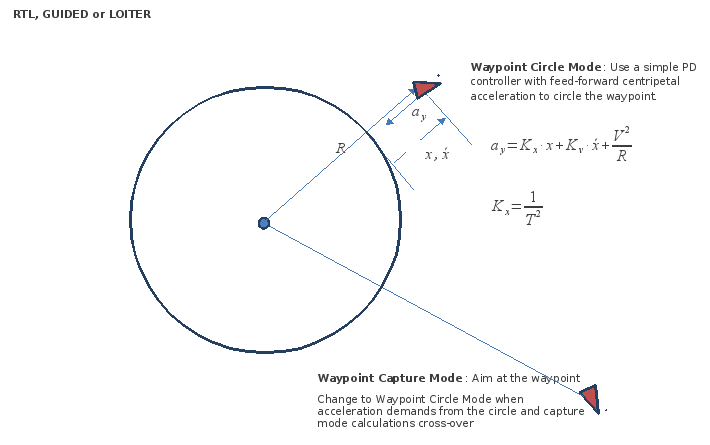
\includegraphics[width=0.8\linewidth]{figs/pd_loiter.png}	
  \caption{PD navigation controller, for circling waypoints. Source: ArduPilot}
  \label{fig:pd_loop}
\end{figure}


\subsection{Navigation: L1 Controller}

%S. Park, J. Deyst, and J. P. How, "A New Nonlinear Guidance Logic for
%Trajectory Tracking," Proceedings of the AIAA Guidance, Navigation and
%Control Conference, Aug 2004. AIAA-2004-4900.
%
%
Since a fixed-wing aircraft usually can't fly in-place, waypoints can be used in two general ways, the aircraft can fly around it in circles, or hit it and then follow to the next one.

In order to circle it, a L1 controller is used. L1 is an adaptative controller designed for trajectory following on aircraft\cite{Park04_GNC}. This technique provides better following of trajectories by taking advantage of the aircraft inertia and geometric properties of the desired path. The controller is briefly explained in figure \ref{fig:l1_loop}.
%
%


\begin{figure}[H]
\centering
  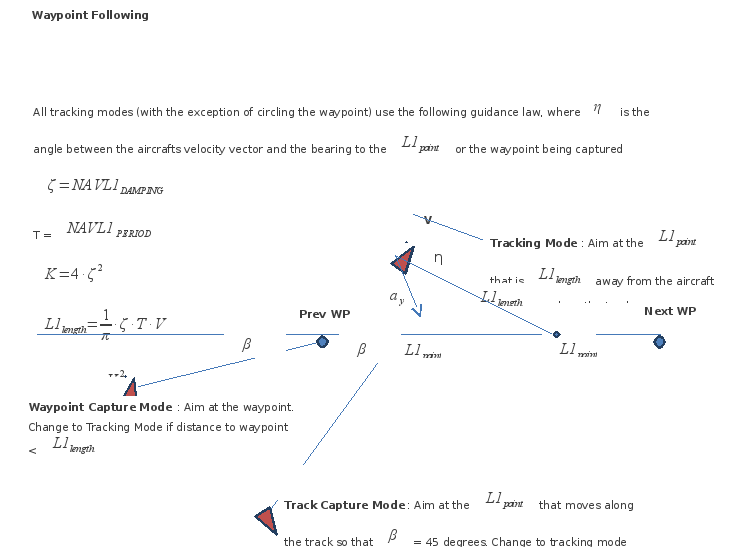
\includegraphics[width=0.9\linewidth]{figs/l1.png}	
  \caption{L1 navigation controller. Source: ArduPilot}
  \label{fig:l1_loop}
\end{figure}

\section{On VTOL Mode}
%
On the VTOL or multirotor mode, cascaded P\footnote{Proportional}/PID\footnote{Proportional-Integral-Derivative} loops are used.
The inner loops control the angular speed, and the outer loops control the attitude, with the outermost loops controlling the altitude and position (again with the L1 controller). These controllers can be seen in figure \ref{fig:copter_attitude_loops}.
\begin{figure}[H]
\centering
  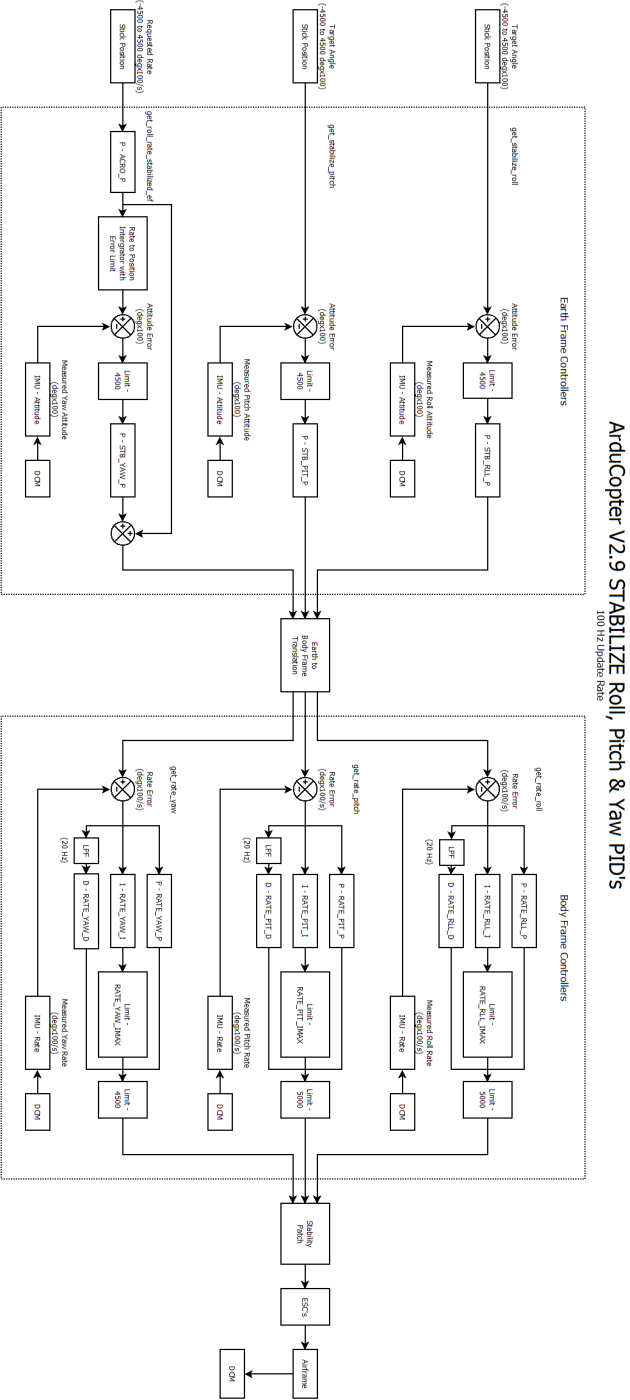
\includegraphics[width=0.65\linewidth]{figs/copterpids.png}
  \caption{Attitude controller. Source: ArduPilot}
  \label{fig:copter_attitude_loops}
\end{figure}


\chapter{Prototyping} \label{chap:prototyping}

As in any product development, a few protoypes were developed.
First a smaller , 50cm wingspan aircraft with no airfoil was assembled to test and tune the flight controllers. The reduced version also enabled testing in close spaces and proximity with people with reduced danger.

With the reduced prototype proven, the larger one, photography-ready was developed. The larger one is closer to the final desired product, and is able to be used as such.

Both prototypes are described, as well as their assemblies, in the next sections.
 


\section{Reduced Scale Prototype}

A reduced prototype was used for preliminary tests of the flight controller and control systems.

Mechanically, this prototype consists of a foam board, two motors, and two control surfaces.

Smaller electronics are used as well. The servos are Turnigy 9 gram servos, The motors are AXN Floater-Jet 2208 2150KV brushless motors, the Escs are HobbyKing's RedBrick 30A ESCs, and the battery a Zippy Compact 3s 1000mah 35C.

The control surfaces were taped to the main body, and linked to the servos by a wire and plastic horn.

The motors had a custom mount 3D-Printed and fitted into the foam.

For the tests and tuning, the prototype had a hook on top, so it could be hang on the ceiling to avoid hitting the floor and walls during the tests.

The first prototype and It's components can be seen on Figure \ref{fig:smallprototypeparts}

\begin{figure}[H]
\centering
  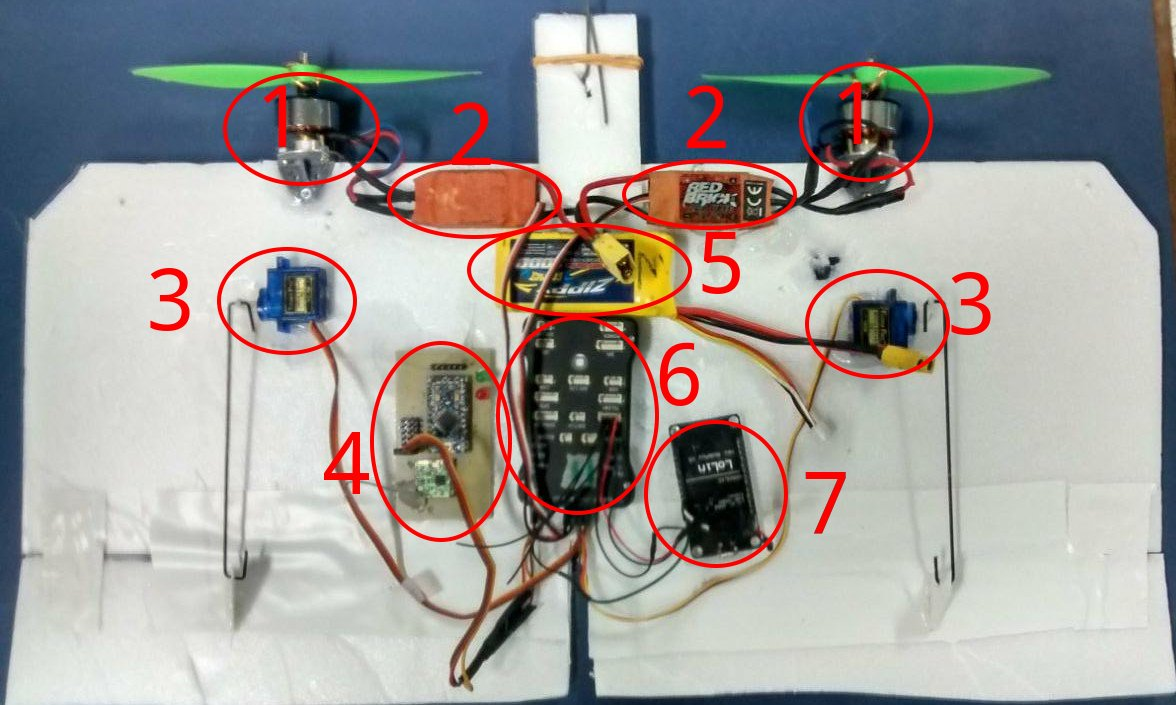
\includegraphics[width=\linewidth]{figs/reducedprototype.jpg}
  \caption{Reduced Prototype and parts:\\
   1 - Motors and 3D-printed mounts\\
   2 - HobbyKing RedBrick 30A ESCs\\
   3 - Turnigy Pro 9 gram servos\\
   4 - Diy OpenLRS 433 MHz receiver\\
   5 - Zippy Compact 3s 1000mAh 35C lithium-polymer battery\\
   6 - Pixhawk controller\\
   7 - ESP-8266 board for telemetry}
  \label{fig:smallprototypeparts}
\end{figure}

\section{Large Prototype}

For the larger prototype, standard RC building and fast prototyping technologies were used.
The Zag12 airfoil at root was 3D printed in 3 parts (Figure \ref{fig:printedairfoil}) then joined and insulated from the hot-wire heat with aluminum foil. For the trapezoidal wings, one side of the wire was tied to a fixed point, in such way that, if the airfoil was a circle, the wire would cut a cone on the foam. This enabled the cut of the trapezoidal wings out of foam. For the center section, two profiles were 3D-printed. their perimeters were then marked with numbers, in such way that two people, one on each side, could coordinate the hot-wire cutting process.

\begin{figure}[H]
\centering
  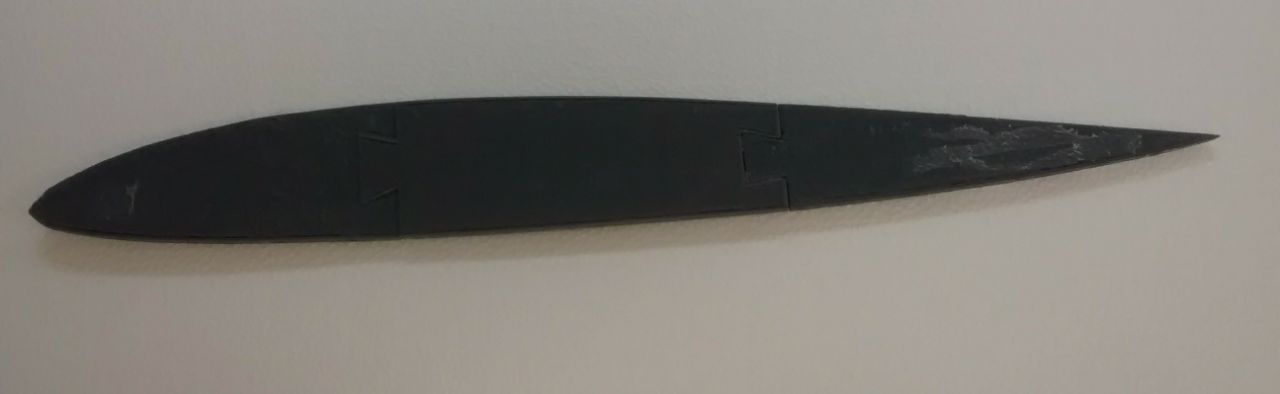
\includegraphics[width=\linewidth]{figs/printedairfoil.png}
  \caption{3D Printed Airfoil}
  \label{fig:printedairfoil}
\end{figure}



This process isn't perfect for the trailing edge, so some of it needs to be removed, which later gets replaced by the elevons.

The cut foam then needs to be sanded down to remove imperfections.
The half-wings are then joined with hot glue, and fiber glass spars are used to reinforce the structure.


From this point, The sections can be joined permanently or spars can be used to quickly assemble them.


With the three sections properly cut, they are glued together and sanded, and glass fiber rods were embedded and glued into the structure, two on the top and two on the bottom.

With the main structure assembled, the servos were embedded into the structure. A pocket was carved with hot wire, and two nut-holding 3D-printed parts were embedded deep into the foam and used to screw the top cover, as seem on the figure \ref{fig:servomount}.


\begin{figure}[H]
\centering
  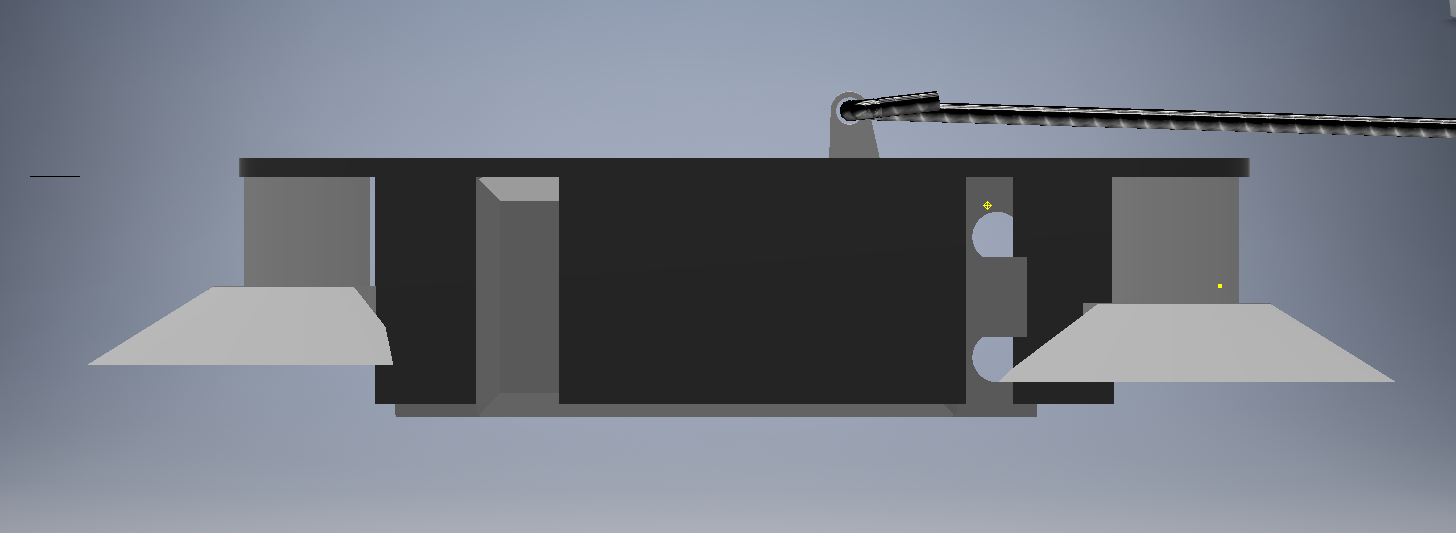
\includegraphics[width=\linewidth]{figs/nutholder1.png}
  \caption{3D-printed servo mount structure.}
  \label{fig:servomount}
\end{figure}


\begin{figure}[H]
\centering
  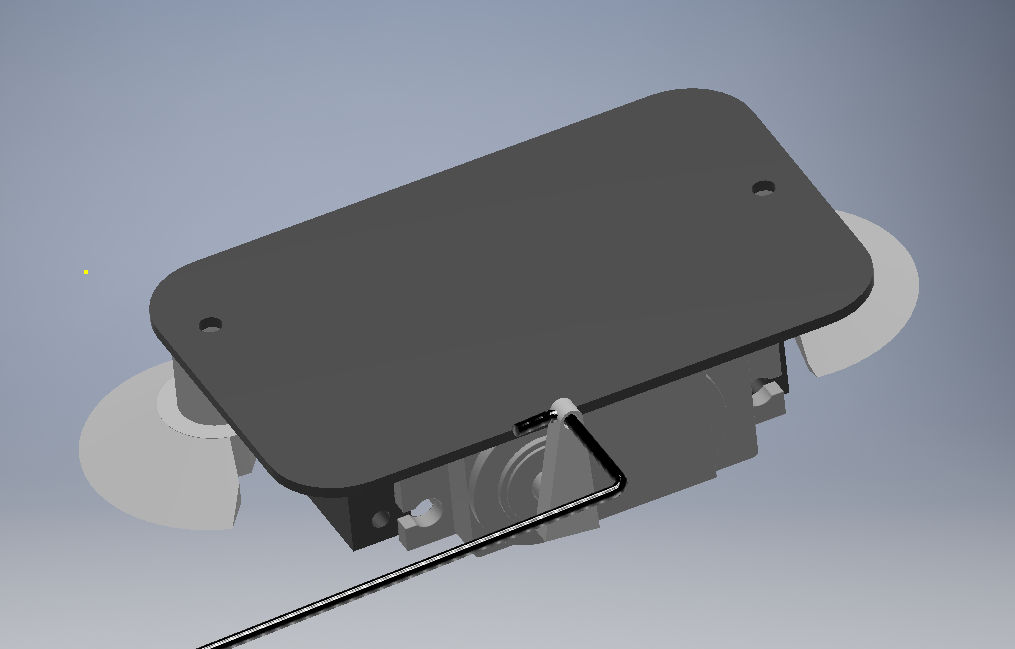
\includegraphics[width=\linewidth]{figs/nutholder2.png}
  \caption{3D-printed servo mount structure.}
  \label{fig:servomount2}
\end{figure}


The main structure was then covered in vinyl, for aesthetical and structural purposes (the tension on the vinyl helps making the structure stiffer). The vinyl is a material that shrinks when heated, which makes it tension itself over it's surface.

The motor mounts were designed so they fit perfectly on the wing profile, and 3D-printed, glued and screwed into the main wing.
The mounts can be seen on figure \ref{fig:motormount}


\begin{figure}[H]
\centering
  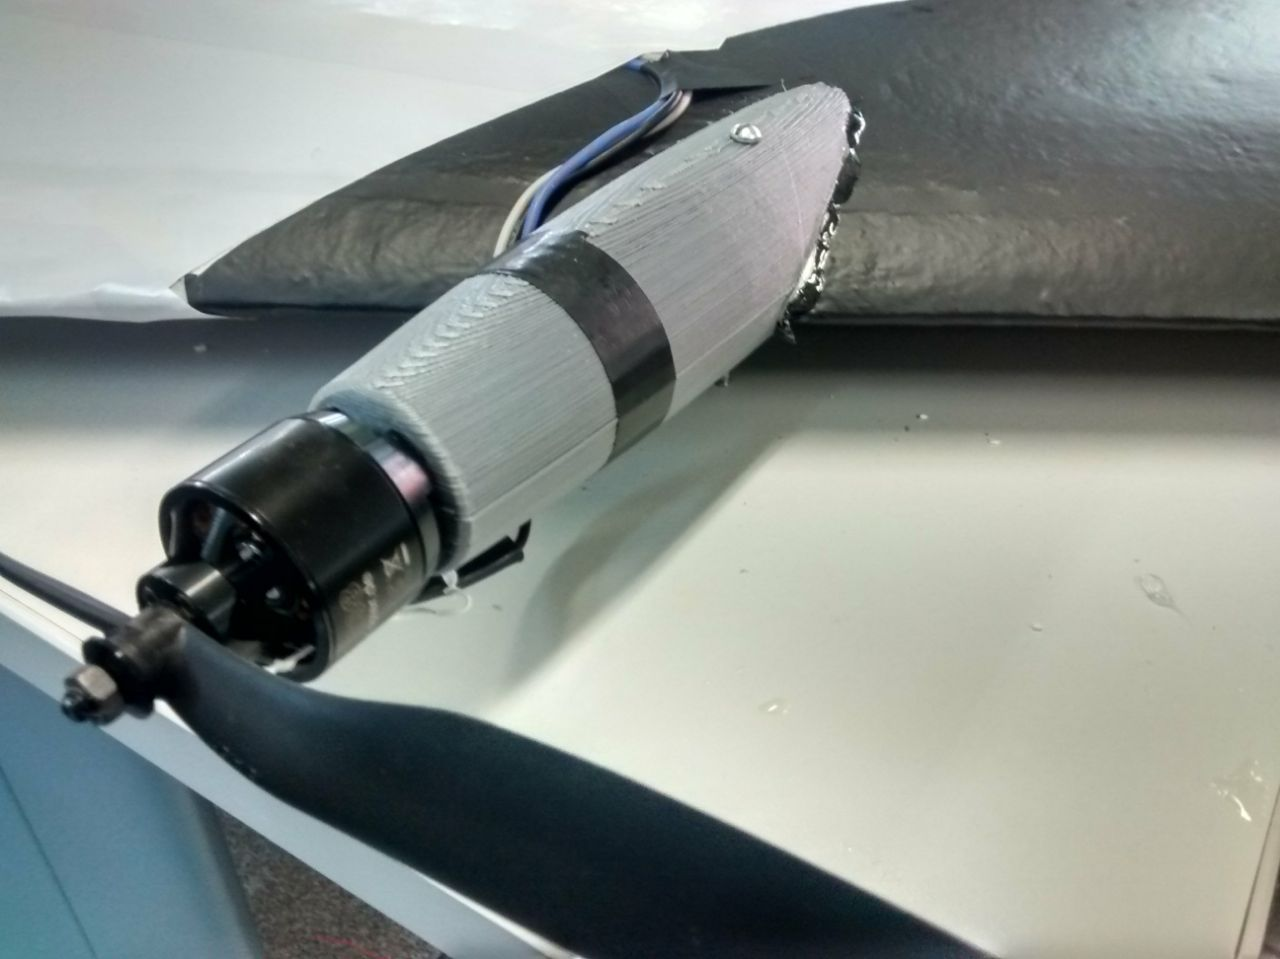
\includegraphics[width=\linewidth]{figs/3dprintedmount.png}
  \caption{3D-printed motor mount structure.}
  \label{fig:motormount}
\end{figure}
	
	
	

 \begin{figure}
\centering
\begin{subfigure}{.5\textwidth}
  \centering
  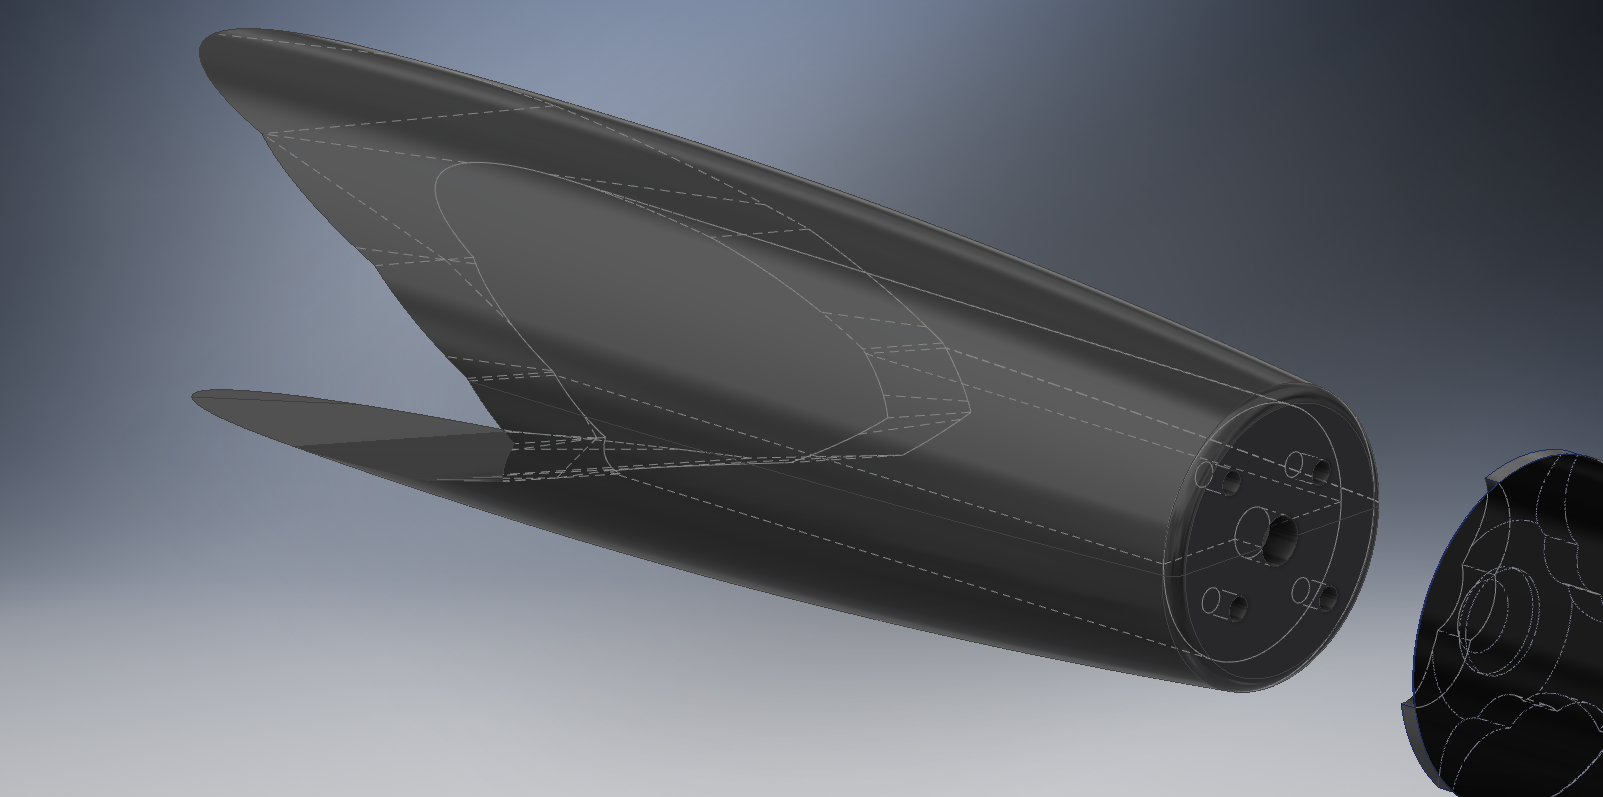
\includegraphics[width=\linewidth]{figs/pods1.png}
  %\caption{Todos os passos do Nelder-Mead}
  
\end{subfigure}%
\begin{subfigure}{.5\textwidth}
  \centering
  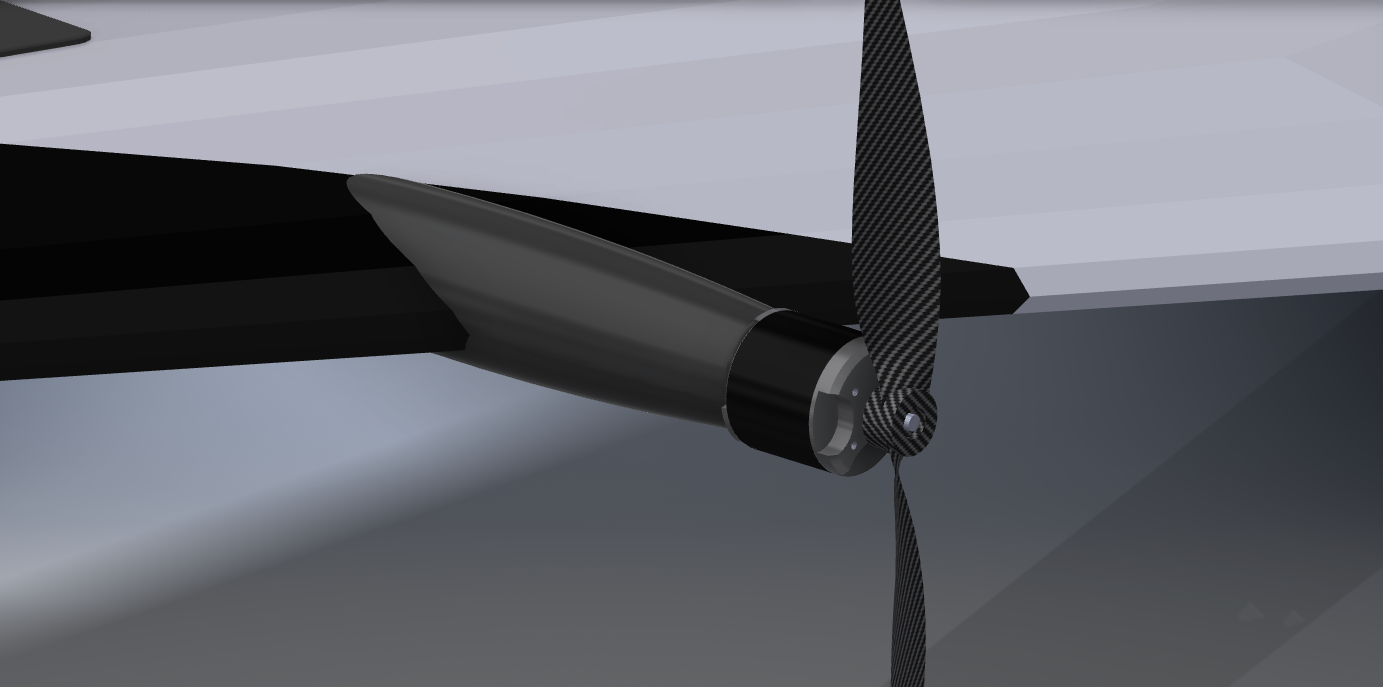
\includegraphics[width=\linewidth]{figs/pods2.png}
  %\caption{Pontos avaliados pelo Nelder-Mead aplicado em um parabolóide.}

\end{subfigure}
\caption{Motor pod design.}
\label{fig:pod}
\end{figure}



The electronics bay was cut using hotwire and carved with a knife. A hot air blower was used to finish the inner surface. The components were placed keeping in mind flexibility to change the camera and batteries without affecting the center of gravity too much, maintaining the approximately the same flight characteristics.

The flight controller was glued with vibration-dampening material. The battery was attached with velcro, and the remaining components are either glued or screwed in place. Special care was taken into keeping the magnetometers away from the motor and battery wires, as the induced magnetic field can adversely affect the magnetic readings.

The hinges were made using a type of fibrous tape. The tape was cut into peaces and glued onto itself, in such way that the piece of tape first sticks on the top section, then on the overlapping sections does not stick at all, and finally, sticks on the bottom.
then these compound tapes are glued in pairs, with one piece sticking on the bottom of the wing and top of the elevon, and the other on the top of the wing and bottom of the elevon. This can be seen on Figure \ref{fig:hinges}.


\begin{figure}[H]
\centering
  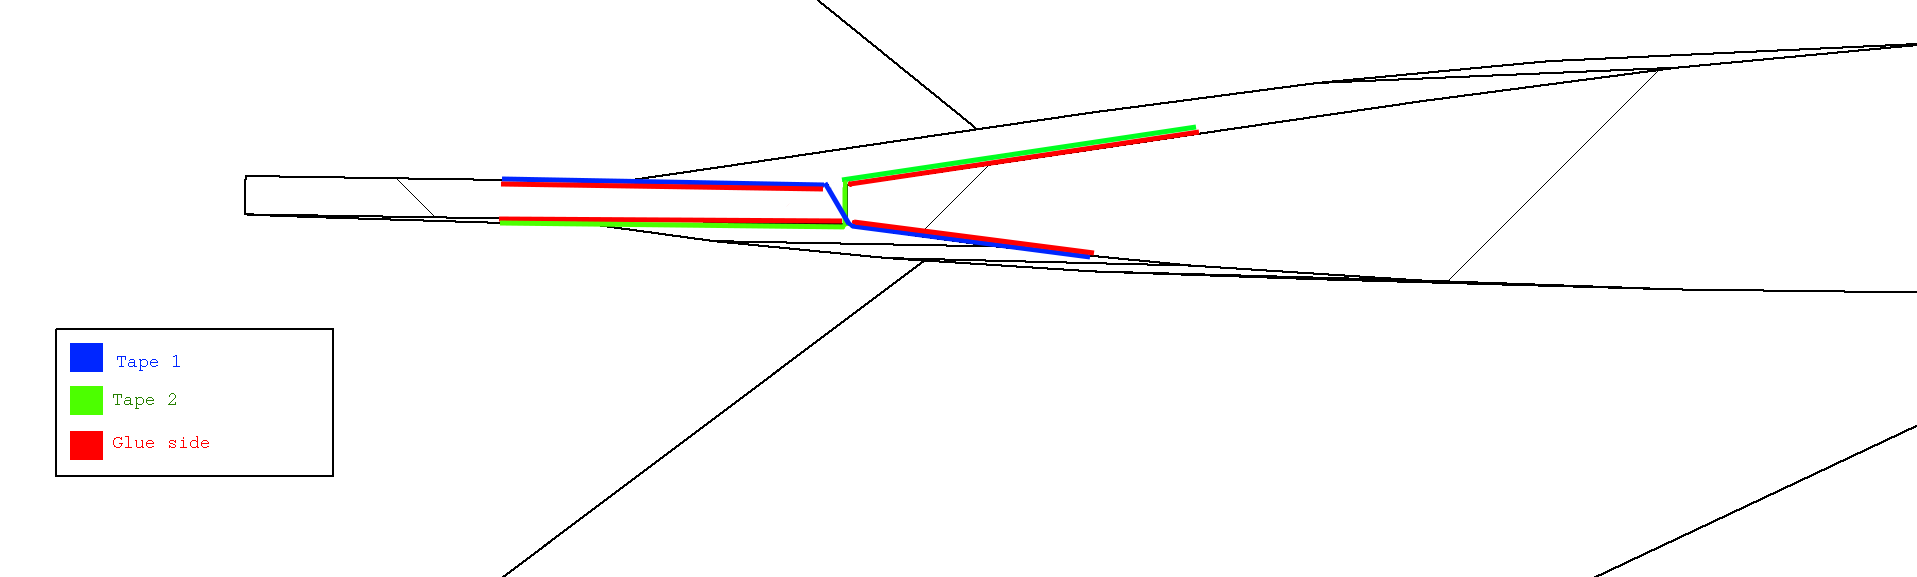
\includegraphics[width=\linewidth]{figs/elevons2.png}
  \caption{hinges setup.}
  \label{fig:hinges}
\end{figure}
	
	
	
The winglets, which usually have only an aerodynamic function, as they increase the yaw ($Z$) stability and help avoid wing tip vortexes, here also need to work as a landing gear in VTOL mode.

As they need to let go after certain amount of force is exerted, and need to be removable to aid in transportation, a magnetic system was idealized. On the wingtip there's a 3D-printed profile with slots for the magnets, and the mirrored profile is also present on the winglet. This profile can be seen on Figure \ref{fig:magnetcoupler}. This profile made sure that four pairs of magnets touch on each winglet. However this design allows slipping between then airfoils,so Velcro was used again to help stiffen the structure, without making it too hard, allowing the winglet to absorb impacts and come loose before damaging the rest of the aircraft.

	
\begin{figure}[H]
\centering
  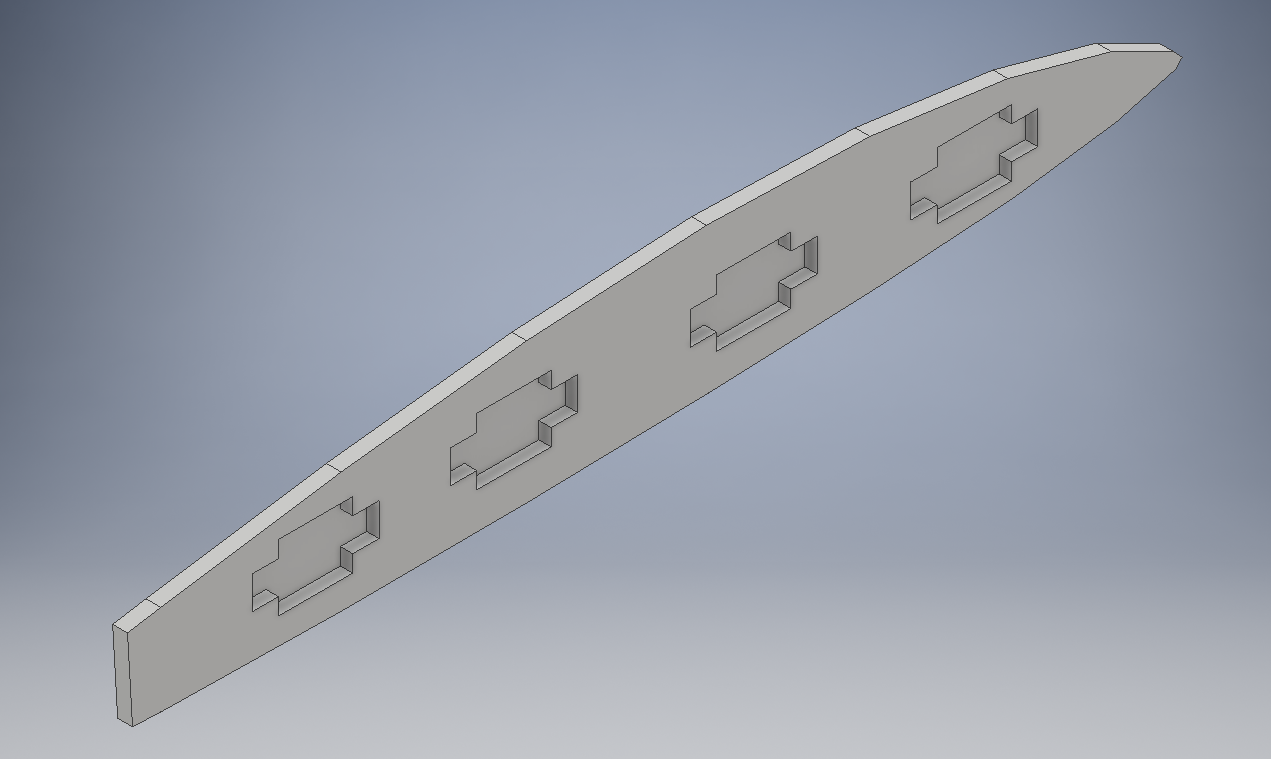
\includegraphics[width=\linewidth]{figs/magnetcoupler.png}
  \caption{3D-printed magnetic coupler.}
  \label{fig:magnetcoupler}
\end{figure}
	

\begin{figure}[H]
\centering
  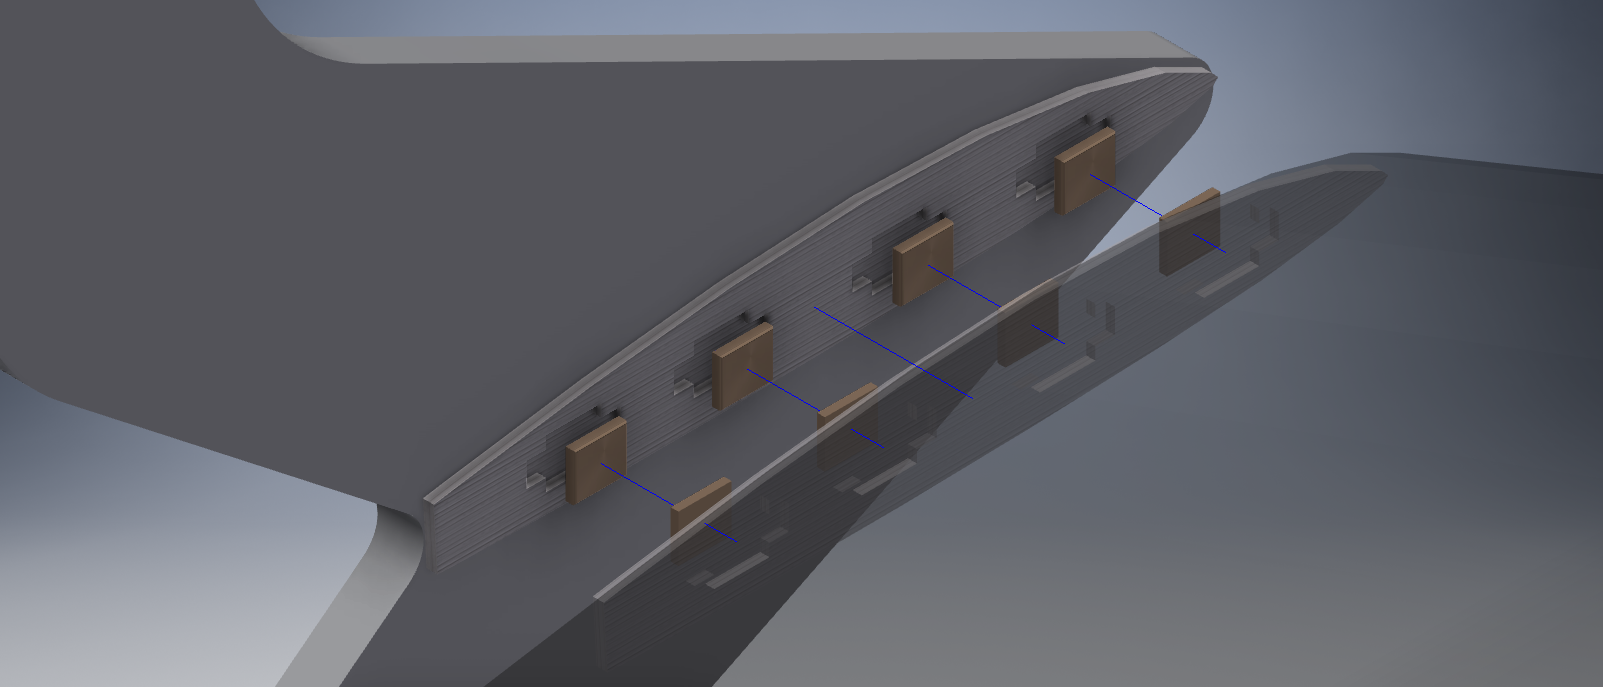
\includegraphics[width=\linewidth]{figs/magnetassembly.png}
  \caption{3D-printed magnetic coupler and winglet assembly.}
  \label{fig:magnetcoupler2}
\end{figure}
	

\section{Software Setup}

In order to use the ArduPilot software stack to control a tailsitter, some setup is necessary. First the regular ArduPilot setup:
\begin{itemize}
\item Frame Type Configuration: The kind of aircraft frame needs to be chosen, in this case, it is a tail sitter. This setups the initial parameters and controllers, as well as output mixers.

\item Compass Calibration: This step performs a calibration on the (in this case) three magnetometers present in the board. Calibrated magnetometers are important for precise heading readings.

\item Radio Control Calibration: This recognizes the PWM ranges sent by the radio, so the flight controller knows when to arm/disarm, or apply full throttle.
\item Accelerometer Calibration: This step calibrates the accelerometer. As the Pixhawk might not be leveled on the frame, calibrating the acelerometers is important to know the aircraft real orientation.
\item ESC Calibration: Just like the flight controller, the ESCs also need to know the full range on the PWM received from the Pixhawk, and thus need calibration;
\end{itemize}

After the basic setup, additional changes need to be done on the parameter level:
\begin{itemize}
\item AHRS\_EKF\_TYPE = 3 This makes the flight controller use an extended Kalman Filter that takes into consideration the accelerometer for translations, not only orientations.

\item ARMING\_CHECK,230 A custom pre-flight check is done, disabling the GPS checks due to the problems reported in \ref{badgps}.

\item SCHED\_LOOP\_RATE = 300 This makes the Kalman filter update at 300 Hz, important for faster responses on multirotor-like aircraft, like this one in VTOL mode.

\item SERVO3\_FUNCTION = 73, SERVO4\_FUNCTION = 74 : This sets outputs 3 and 4 to output the mixers of left motor and right motor on a dual-motor tail sitter aicraft.

\end{itemize}

%\section{Control Tuning}



\section{Troubleshooting}

This section details some of the problems faced during this work and how each of them was handled.

\subsection{The Electronic Speed Controllers Do Not Work}
With The hardware setup, it was noted that the ESCs did not respond to the flight controllers. This could be due to two main reasons:
\begin{itemize}
\item The ESCs are unable to cope with the 400Hz PWM \footnote{Pulse Width Modulation} signal generated by the flight controller;
\item The signal voltage was not high enough;
\end{itemize}

The ESCs did answer properly to a 50Hz signal, so they were working.
%
It was later found in the DiyDrones\cite{diydronesesc} forum that the ESCs are incompatible with the Pixhawk controller, and two components had to be removed for them to work.
%
Upon further inspection, the components were noticed to be a resistor and a capacitor. This is a strong indication of an RC filter. The presence of an RC filter on the inputs, coupled with the output resistance present in most flight controllers signal outputs, resulted in a resistive divider, as seem on figure \ref{fig:divider}.
This effectively lowered the voltage read on the microcontroller to 2, as seen on figure \ref{fig:lowvoltage}.
Further inspection showed that only one 512 (5100 $\Omega$ ) resistor was present on the board, and it was, along with a capacitor, bridging a route to ground.
The removal of these components was enough to raise the read signal value to 3.4 V, solving the issue, as seem on Figure \ref{fig:highvoltage}.

With the ESCs accepting their input signals, they needed calibration. The calibration of an RC ESC is a process where it learns the high and low bounds on it's input signals. The ESC is turned on with the maximum possible input, it beeps, and the signal can be lowered to the minimum, then it beeps again.


\begin{figure}[H]
\centering
  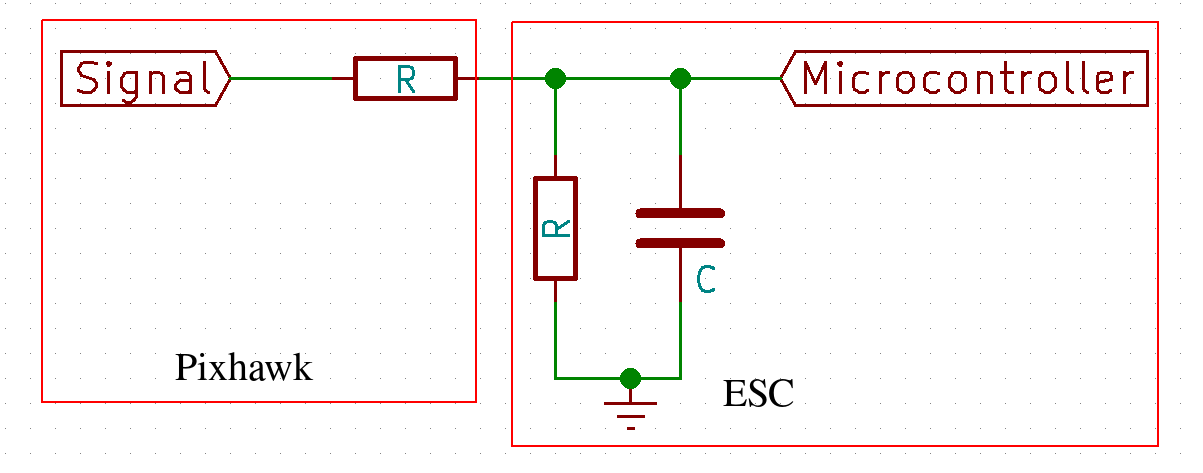
\includegraphics[width=\linewidth]{figs/divider.png}
  \caption{Schematic of signal path between Pixhawk and ESC.}
  \label{fig:divider}
\end{figure}
	
\begin{figure}[H]
\centering
  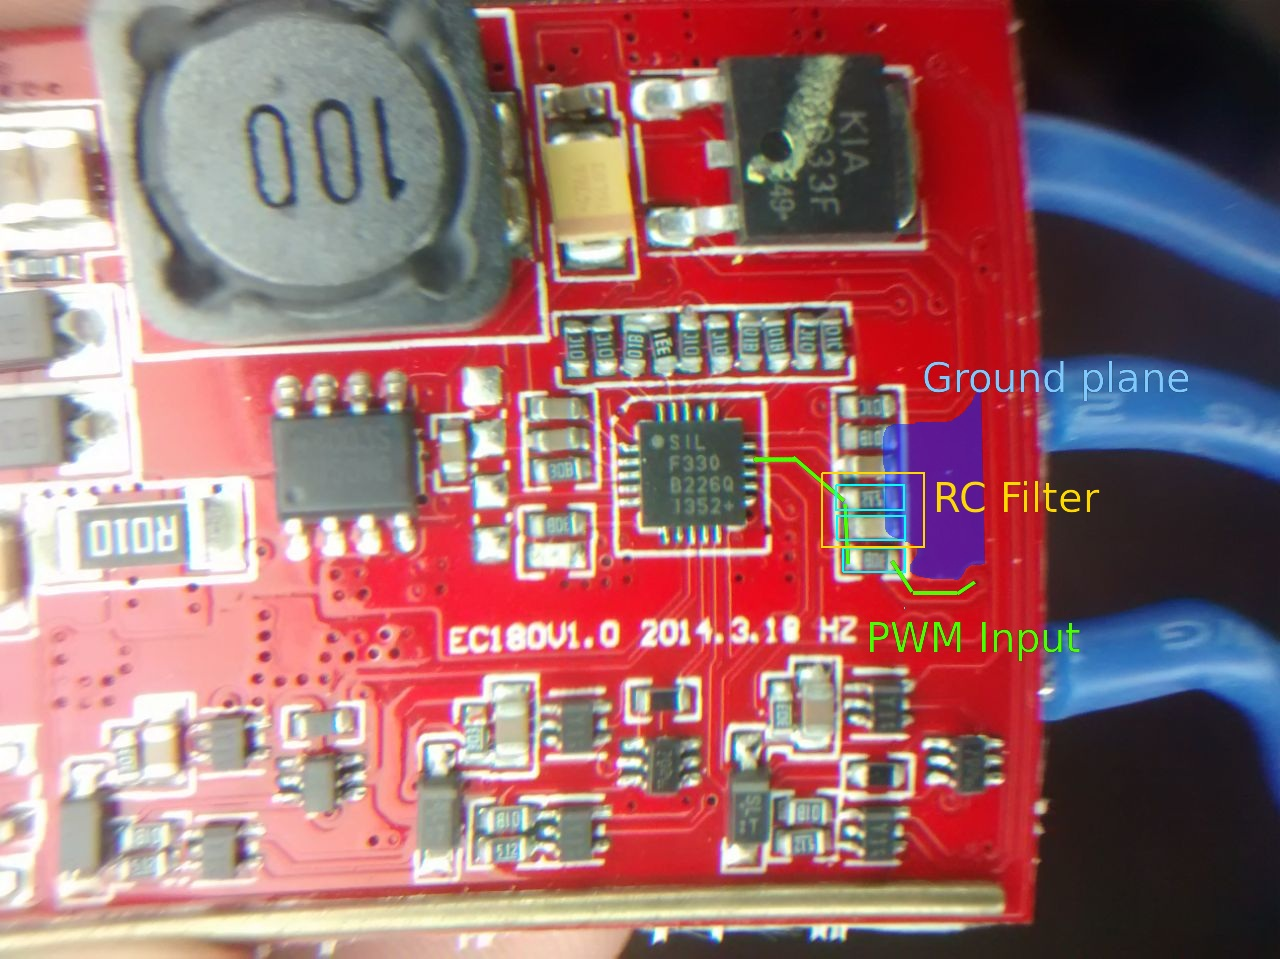
\includegraphics[width=0.7\linewidth]{figs/escbeforeschematic.jpg}
  \caption{Schematic overlaid on ESC board.}
  \label{fig:divider2}
\end{figure}
	


\begin{figure}[H]
\centering
\begin{subfigure}{.5\textwidth}
  \centering
  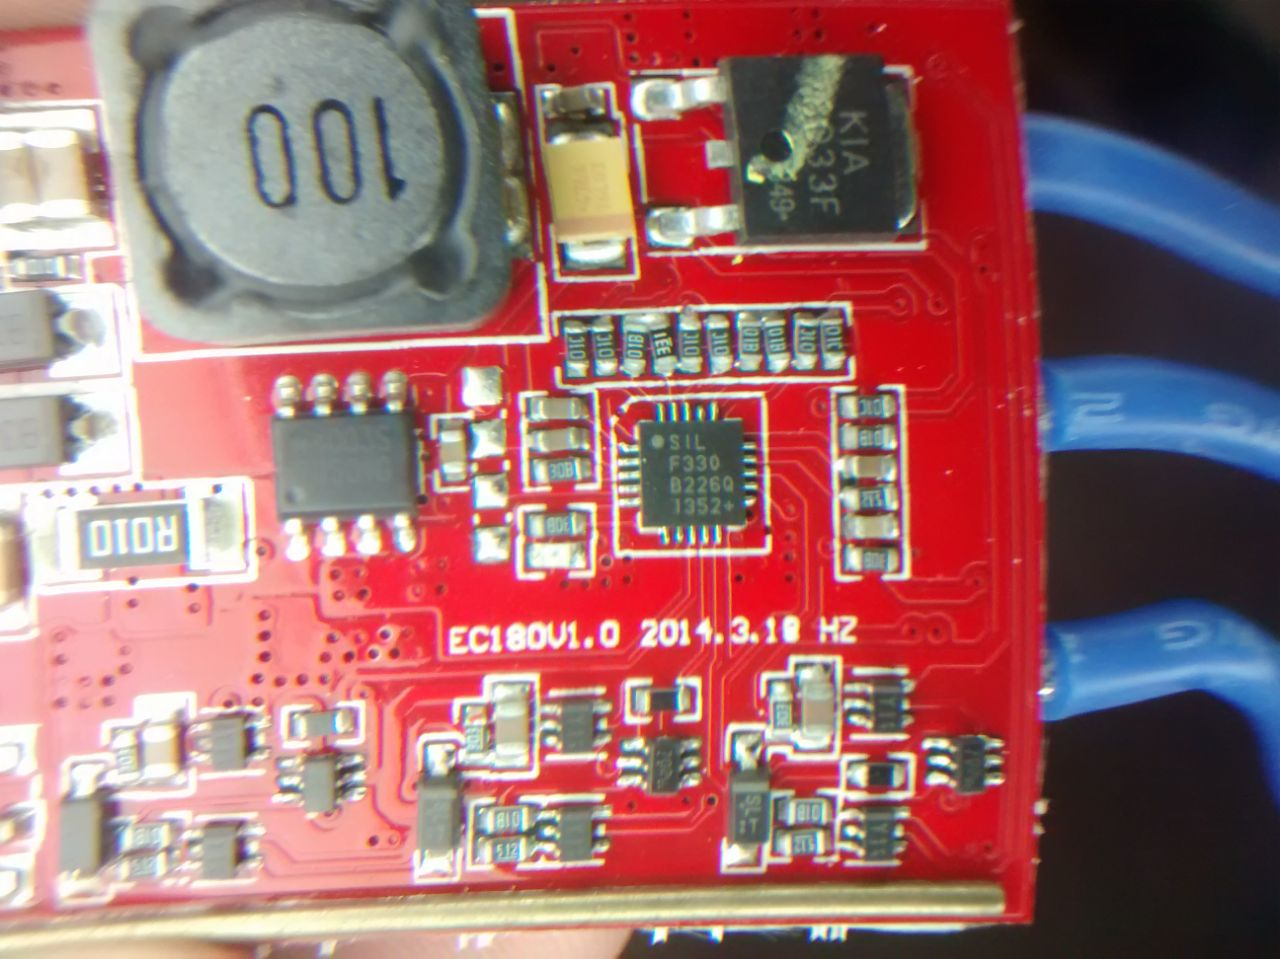
\includegraphics[width=\linewidth]{figs/escbefore.jpg}
\caption{ESC before modification.}
\end{subfigure}%
\begin{subfigure}{.5\textwidth}
  \centering
  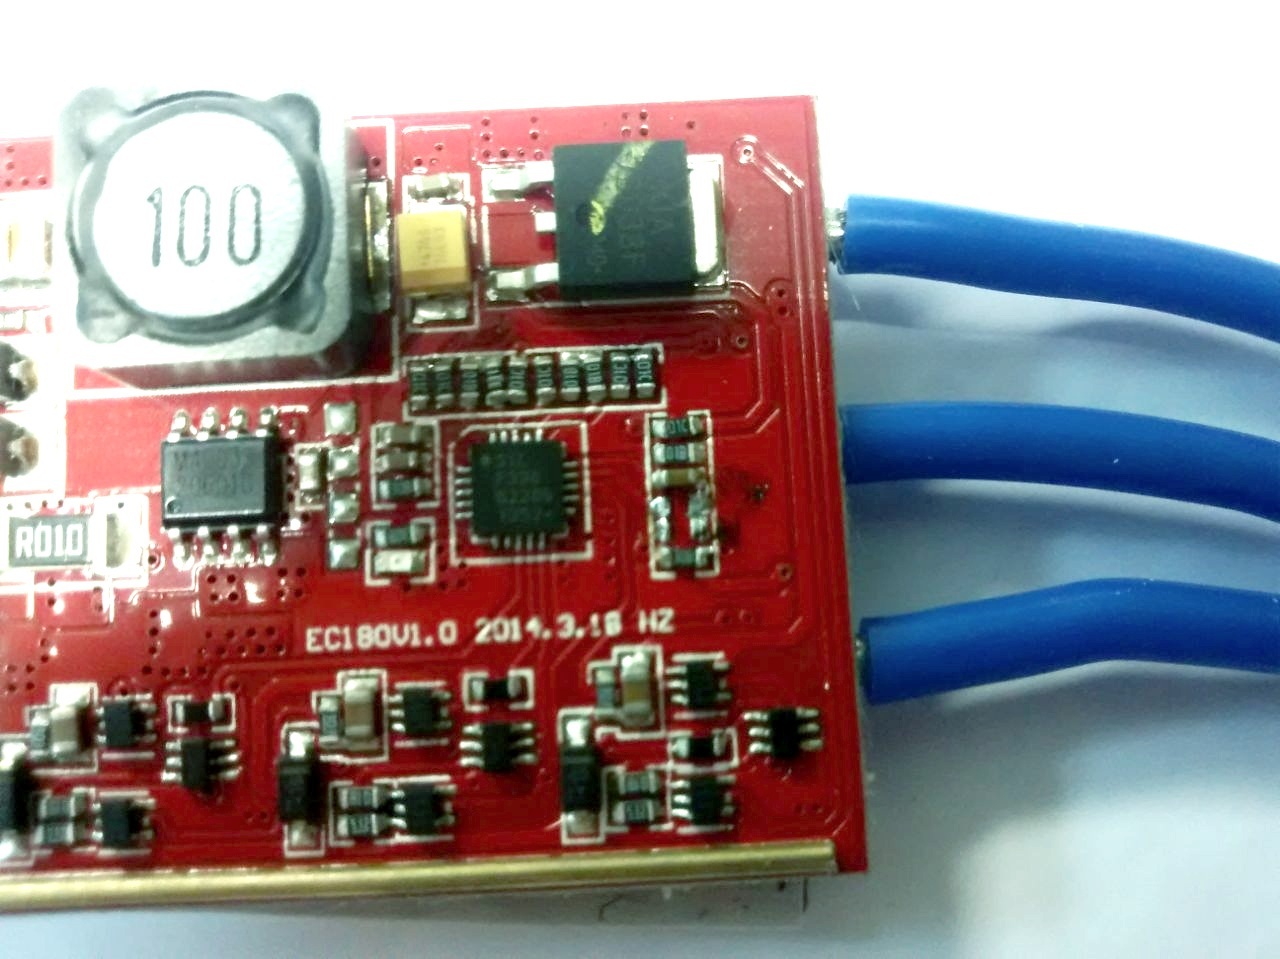
\includegraphics[width=\linewidth]{figs/escafter.jpg}
  \caption{ESC after modification.}
\end{subfigure}

\begin{subfigure}{.5\textwidth}
  \centering
  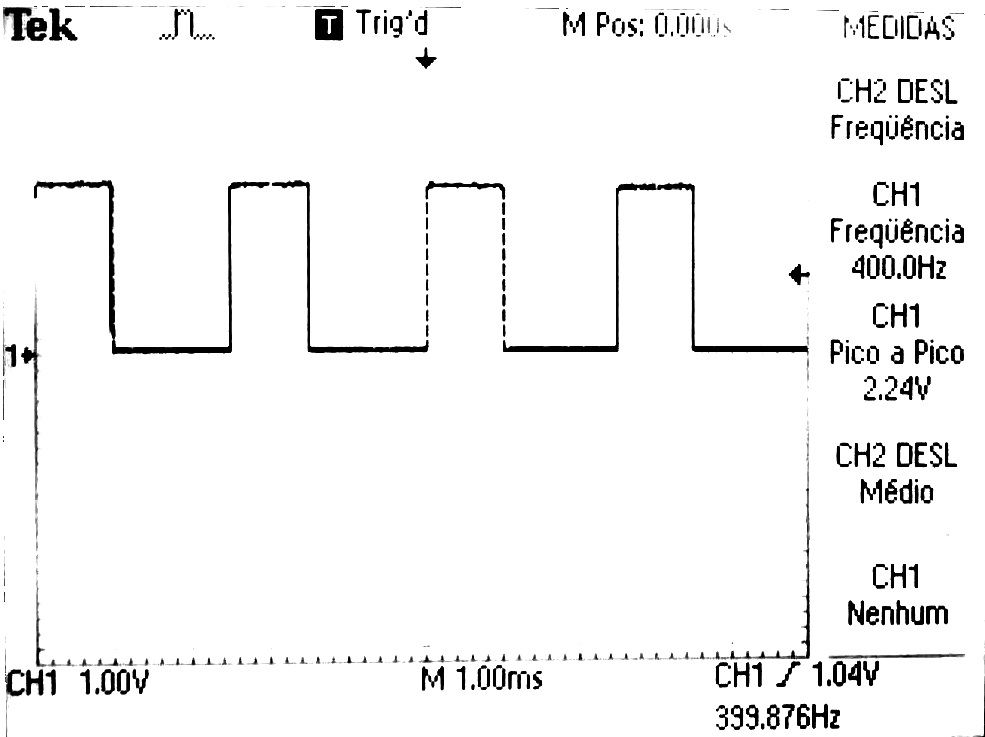
\includegraphics[width=\linewidth]{figs/sinalruim.jpg}
  \caption{Signal before modification.}
  \label{fig:lowvoltage}
\end{subfigure}%
\begin{subfigure}{.5\textwidth}
  \centering
  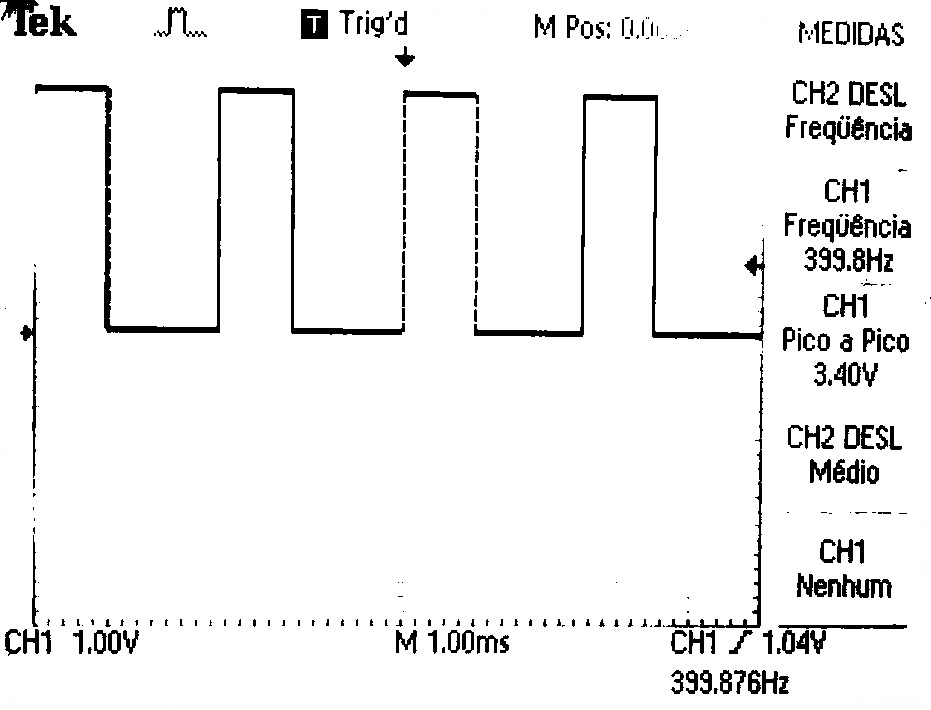
\includegraphics[width=\linewidth]{figs/sinalbom.jpg}
  \caption{Signal after modification.}
    \label{fig:highvoltage}
\end{subfigure}

\caption{Modifications on the ESC.}
\label{fig:neldermeadsteps}
\end{figure}

\subsection{The Elevons Have a High Frequency Pitch oscillation}
Even on the ground, activating the stabilization control resulted in increased high-frequency oscillations of the control surfaces on the pitch direction.
%
Any minor servo correction caused a small movement on the aircraft body, due to moment conservation. This movement is detected and, when trying to compensate this behavior repeated until the oscillation peaked with the maximum amplitude reachable by the servos.
%
This behavior was linked to the the derivative terms on the pitch controllers.
%
Since, as seem on picture \ref{fig:roll_loop}, the roll and pitch controls are attenuated with the throttle, this effect is not present during flight. This effect should be handled in software in the futures, but was not prejudicial to the tests in this project.

\subsection{Bad GPS Health}
\label{badgps}
The GPS used, even though recognized by the flight controller, made it show "Bad GPS Health messages". Further research showed that the board was a badly manufactured clone\cite{badgps}, where the wrong version of the EEPROM chip was used, with a different pinout, meaning that while the flight controller was able to communicate and setup the GPS, it was unable to perform a warm start, which is looking for the right satellites using it's last known position saved on the EEPROM.

This issue has three possible solutions:
\begin{itemize}
\item Unsolder the chip and resolder to the right connections with wires.
\item Replace the chip with the correct one.
\item Replace the whole GPS for a working one.
\end{itemize}

The latter was chosen as there was a spare one available, requiring only re-wiring.
\chapter{Assessment} \label{chap:assessment}

The assessment was incremental. First, the aerodynamic properties were tested on a manual flight, qualitatively, regarding properties such as stall angle, stall speed, and equilibrium point in flight. Following this, the hover capabilities were tested, such as altitude and attitude control. With the basic flight capabilities proven, a few autonomous, test flights were performed, without VTOL. Finally, its VTOL capabilities were benchmarked. These tests are better described, as well as their results, in the following sections.


\section{Tethered Attitude Control Test}

To test the attitude control and stabilization, the prototype was hang by a rope, so it's range of movement was restricted, and it was safer to test indoors.
%
The first tests were qualitative. The wing was armed on the QStabilize mode, where the gyroscope and accelerometer are used to try to maintain the aircraft leveled in VTOL mode (propellers spinning parallel to ground).
%
The expected result was that the elevons should move trying to stop the movement, even without propellers on the motors (again, for safety reasons).
%
The aircraft successfully reacted to disturbances on it's attitude by moving the control surfaces appropriately.


\section{Un-tethered Attitude Control Test} 

For this test, the wing was taken to an open field on the university.
%
For the take-off, it had to be oriented so the wind blew parallel to it's surface, so that the wind didn't flip it over.
%
Take-off cant be too slow, as the winglets adhere to the the ground and can cause the aircraft to tip over.
%
once in the air, the controls and stabilization were good, but once the wind it the aircraft, it turned it perpendicular to the direction of the wind, and the control authority was not enough for both stabilizing flight and turning the yaw axis.
%
While this problem limits the yaw controllability in VTOL mode, the position control is not necessarily affected, as the aircraft can still move in a mixed attitude between VTOL and fixed wing, inclined against the wind and maintaining position.
%

This could possibly be fixed by increasing the winglets area, however this also increases the area the wind hits, and needs more testing to verify.
%
Another possibility is tweaking the pitch angle limits, which by default are $\pm 30\degree$, in this case was not enough to fight the wind.

The flight path can be seen on Figure \ref{fig:flight1-3d}, and an in-flight photo on Figure \ref{fig:flight1-photo}. The video is available on youtube\cite{flight1}.
%
No attempt at transitioning to fixed-wing mode was made at this flight due to the reduced space available, which made the pilot feel unsafe.
	

\begin{figure}[H]
\centering
  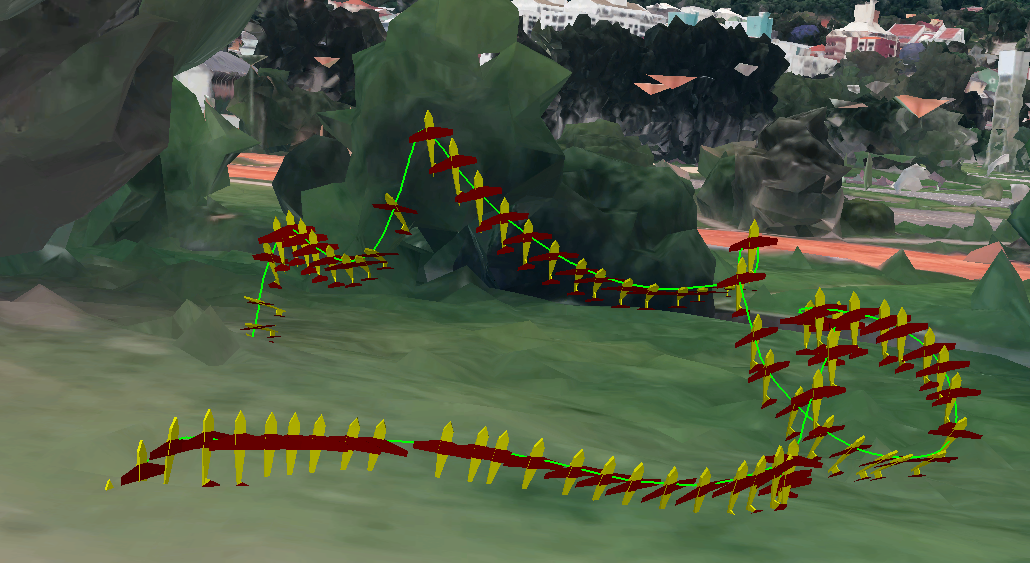
\includegraphics[width=0.7\linewidth]{figs/flight1-3d.png}
  \caption{Visualization of first test flight.}
  \label{fig:flight1-3d}
\end{figure}
	
	\begin{figure}[H]
\centering
  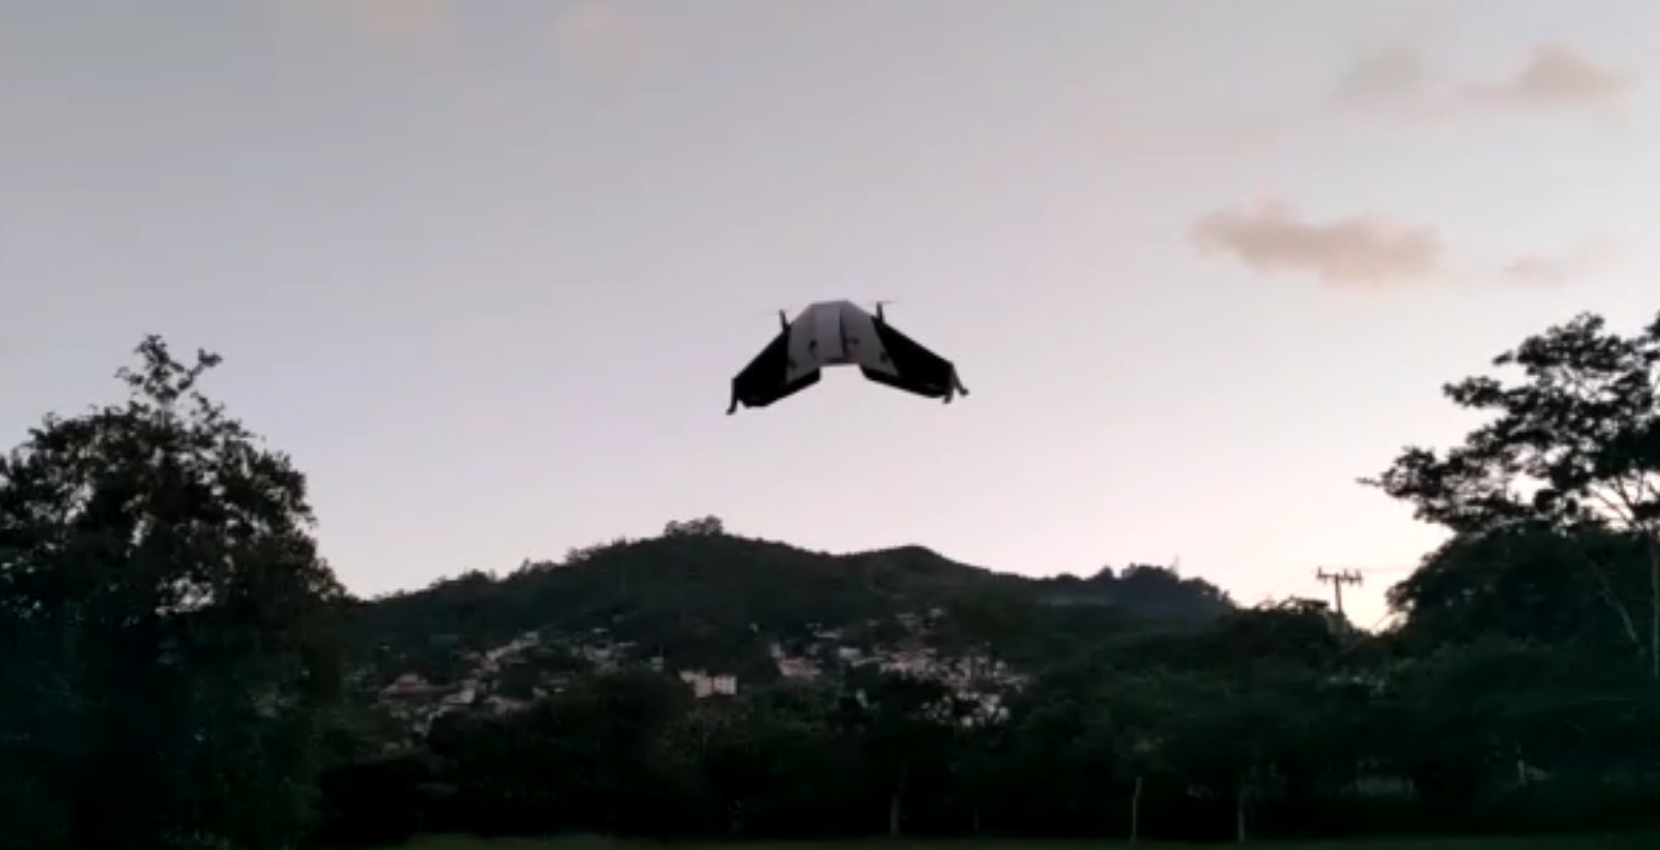
\includegraphics[width=0.7\linewidth]{figs/flight1-photo.png}
  \caption{Photo of first test flight.}
  \label{fig:flight1-photo}
\end{figure}
	



\section{Position Hold}
The next test was taking-off and landing autonomously. Due to the winds and undersized landing gear, the aircraft was positioned with the surface again parallel to the wind flow.

The autonomous take-off however, tried to take-off too slowly, and the winglet/landing gear grip to the grass limited pitch control prior to taking-off, causing the wing to tip over. The solution was to take-off manually, in QStabilize (Quadplane Stabilize) mode, then switching to QLoiter. Five of such flights were attempted. The results are on Table \ref{table:loiter}.

While most of the results were good, a roll oscillation was present on some of the flights, causing instability and forced landings.
The problem appears to be being caused by the navigation controller, as the roll("ATT.Roll") actually follows the roll setpoint("ATT.DesRoll"), who is oscillating, as seem on picture \ref{fig:rollOscillation}. This could mean that the navigation controller is oscillating fast around the given point, with increasingly high amplitude, requiring further tuning of it's parameters. 

	\begin{figure}
\centering
  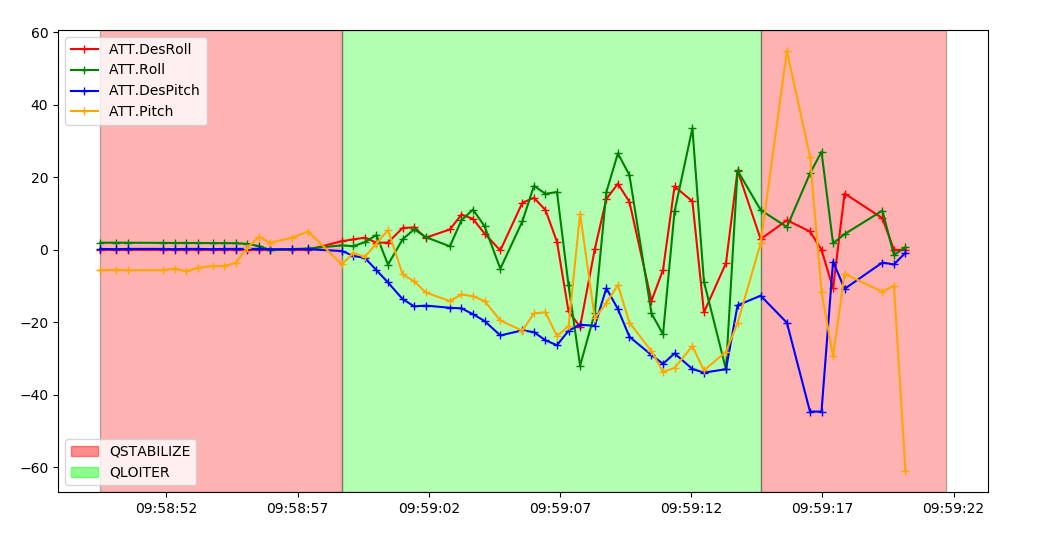
\includegraphics[width=0.9\linewidth]{figs/rolloscillation.png}
  \caption{Visualization of logged attitude control.}
  \label{fig:rollOscillation}
\end{figure}
	


\begin{table}[]
\centering

\resizebox{\textwidth}{!}{%
\begin{tabular}{@{}rrrrl@{}}

Test \# & Flight Time (s) & \begin{tabular}[c]{@{}r@{}}Position \\ Hold Radius (m)\end{tabular} & \begin{tabular}[c]{@{}r@{}}Maximum \\ Altitude (m)\end{tabular} & Notes              \\ \midrule
1       & 47              & 1.5                                                                 & 14.4                                                            &                    \\
2       & 47              & 8.1                                                                 & 12.0                                                            & Roll oscillation    \\
3       & 56              & 3.0                                                                 & 13.1                                                            &                    \\
4       & 37              & 3.7                                                                 & 4.3                                                             & Roll oscillation    \\
5       & 51              & 7.5                                                                 & 13.9                                                            & Pushed by the wind
\end{tabular}%
}
\caption{Loiter tests summary.}\label{table:loiter}
\end{table}


\chapter{Conclusions} \label{chap:conclusions}


% ----------------------------------------------------------
% Finaliza a parte no bookmark do PDF
% para que se inicie o bookmark na raiz
% e adiciona espaço de parte no Sumário
% ----------------------------------------------------------
\phantompart

% ---
% Conclusão
% ---
%\chapter{Conclusão}
% ---

% ----------------------------------------------------------
% ELEMENTOS PÓS-TEXTUAIS
% ----------------------------------------------------------
\postextual
% ----------------------------------------------------------

% ----------------------------------------------------------
% Referências bibliográficas
% ----------------------------------------------------------
\bibliography{bibli}{}

% ----------------------------------------------------------
% Glossário
% ----------------------------------------------------------
%
% Consulte o manual da classe abntex2 para orientações sobre o glossário.
%
%\glossary


%\include{anexos}
%---------------------------------------------------------------------
% INDICE REMISSIVO
%---------------------------------------------------------------------
\phantompart
\printindex
%---------------------------------------------------------------------

\end{document}
